
% ------------------------ Prototype ------------------------

\section*{APPENDIX A - Prototype \label{sec:proto}}
\addcontentsline{toc}{section}{APPENDIX A - Prototype}


\begin{comment}

    Provide the filtered part of RM showing selected features for prototype building. State the detailed steps of compilation, execution and setups. Specify prototype details showing codes, screens, test data, sample output and detailed steps of compilation, execution and setups (if any).

\end{comment}

% ---------- Start the prototype appendix
\noindent
Below are the flow diagrams for the various options that the web application provides.

\begin{figure}[h!]  
    \centering
    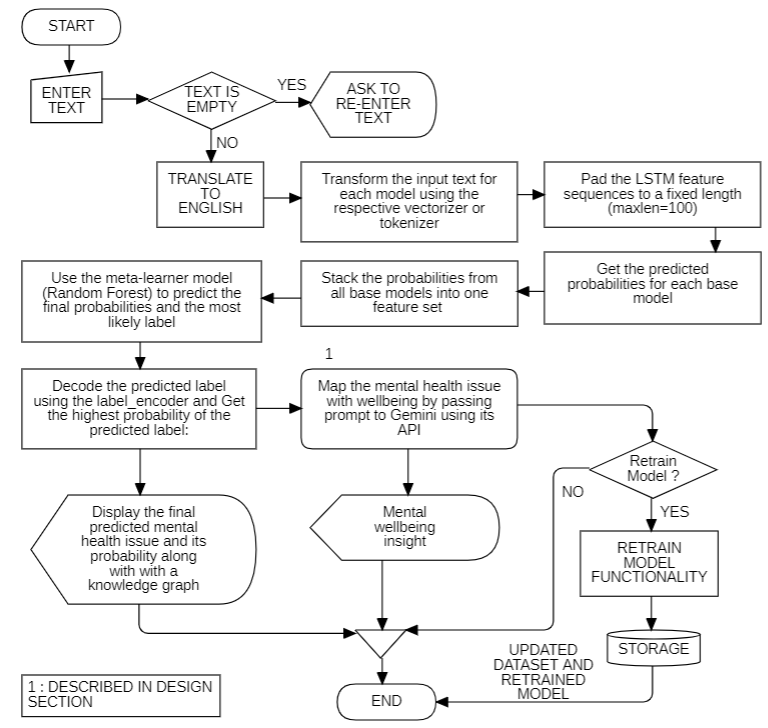
\includegraphics[width=0.72\textwidth]{Images/APP TEXT OPTION.png}  
    \caption*{Text Classification Flow Diagram}
    \label{012i}  % Label for referencing the figure
\end{figure}

% -- pdf upload
\begin{figure}[h!]  
    \centering
    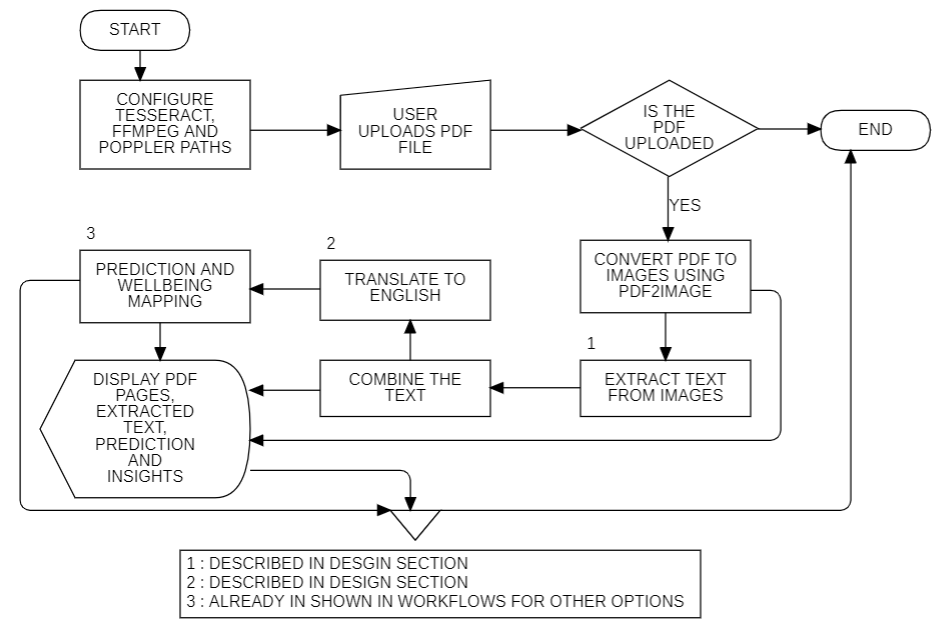
\includegraphics[width=0.72\textwidth]{Images/APP PDF.png}  
    \caption*{PDF Upload Flow Diagram}
    \label{01234i}  % Label for referencing the figure
\end{figure}

\pagebreak

\begin{figure}[h!]  
    \centering
    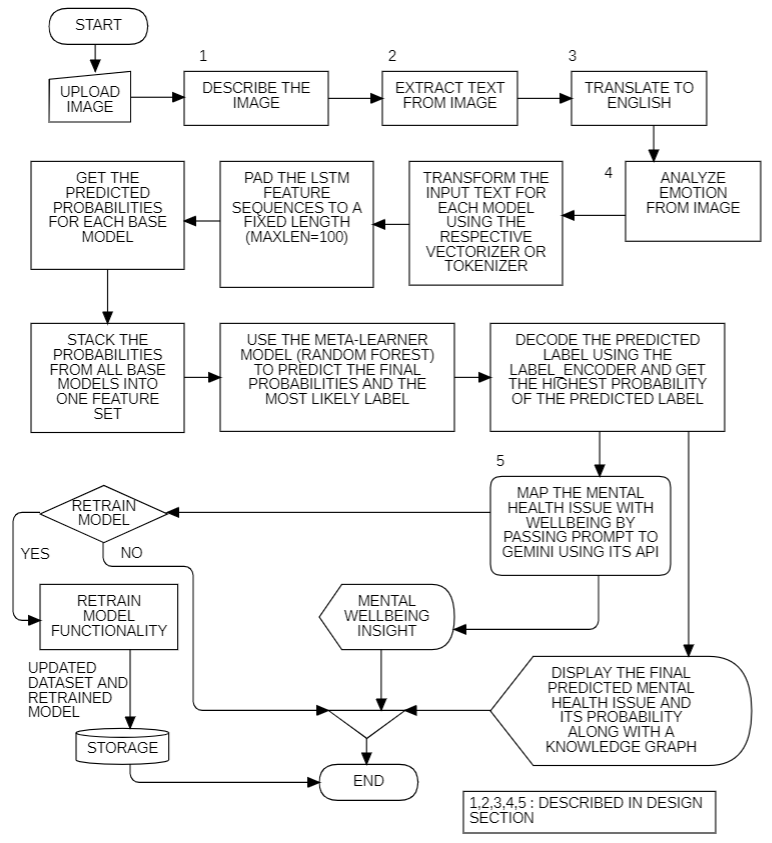
\includegraphics[width=0.72\textwidth]{Images/APP IMAGE OPTION.png}  
    \caption*{Image Classification Flow Diagram}
    \label{011232i}  % Label for referencing the figure
\end{figure}

% -- user response to image
\begin{figure}[h!]  
    \centering
    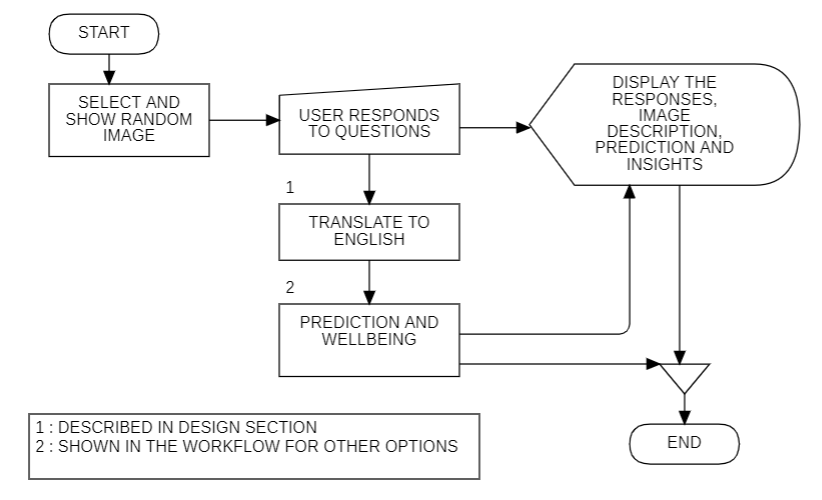
\includegraphics[width=0.72\textwidth]{Images/APP RESPOND.png}  
    \caption*{User Response to Image Flow Diagram}
    \label{01234i}  % Label for referencing the figure
\end{figure}

\pagebreak

\begin{figure}[h!]  
    \centering
    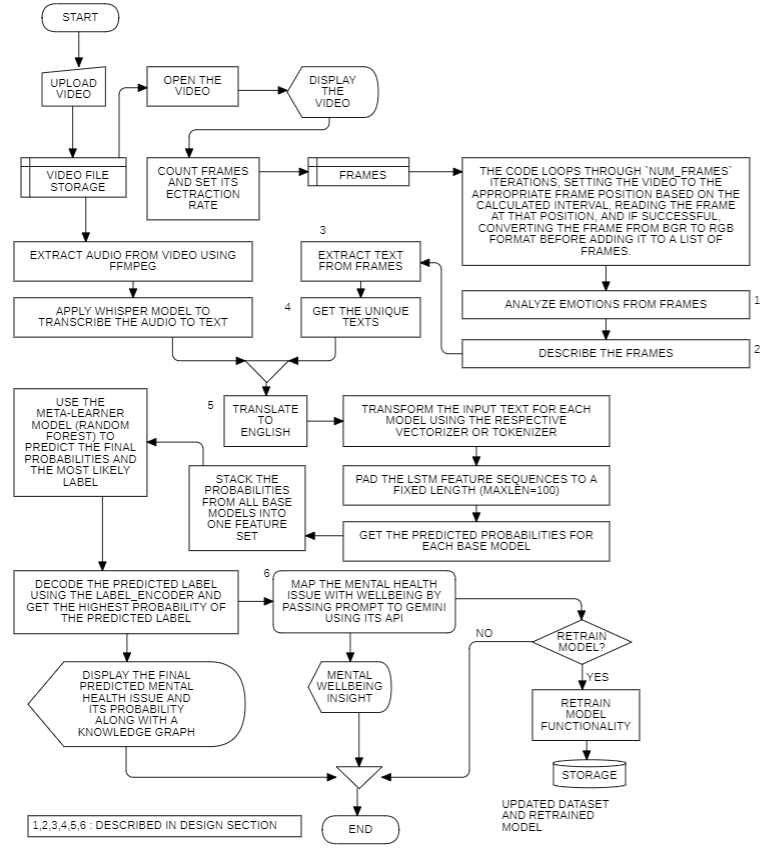
\includegraphics[width=1.0\textwidth]{Images/APP VIDEO OPTION.png}  
    \caption*{Video Classification Flow Diagram}
    \label{01332i}  % Label for referencing the figure
\end{figure}

\pagebreak
\begin{figure}[h!]  
    \centering
    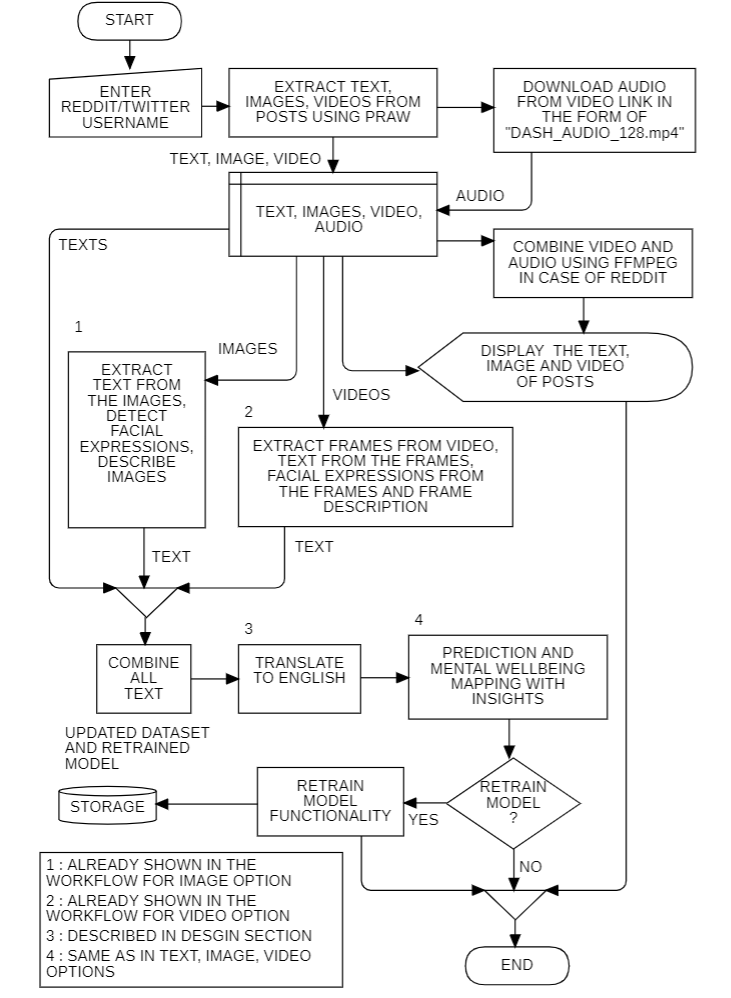
\includegraphics[width=0.9\textwidth]{Images/APP REDDIT.png}  
    \caption*{Reddit and Twitter username Classification Flow Diagram}
    \label{01234i}  % Label for referencing the figure
\end{figure}


\pagebreak
% -- add threer flow diagrams here






\pagebreak

% -- well being survey and calculation

\begin{table}[H]
    \caption*{Step-by-Step Algorithm for the Well-being Survey Option}
    \label{tab:algorithm}
    \begin{tabularx}{\textwidth}{|l|X|X|}
    \hline
    \textbf{Step} & \textbf{Operation} & \textbf{Description / Formula} \\ \hline
    1 & \textbf{Initialization:} \newline
    - Define file paths: \texttt{csv\_file\_path}, \texttt{image\_path}, \texttt{am\_file\_path}. \newline
    - Display title \textit{``Well-being Survey''}. & -- \\ \hline
    2 & \textbf{Display Introductory Image:} \newline
    - Check if the image file exists at \texttt{image\_path} and display it. & --\\ \hline
    3 & \textbf{Display Instructions:} \newline
    - Present informational messages and detailed instructions. \newline
    - Describe the Ryff Scale & 
    \[
    \begin{array}{l}
    \textbf{1} \quad \rightarrow \quad \text{Strongly Disagree} \\
    \textbf{2} \quad \rightarrow \quad \text{Disagree} \\
    \textbf{3} \quad \rightarrow \quad \text{Slightly Disagree} \\
    \textbf{4} \quad \rightarrow \quad \text{Slightly Agree} \\
    \textbf{5} \quad \rightarrow \quad \text{Agree} \\
    \textbf{6} \quad \rightarrow \quad \text{Strongly Agree}
    \end{array}
    \]
    \\ \hline
    4 & \textbf{Load or Create Response Data:} \newline
    - Attempt to load \texttt{response.csv} into a DataFrame. \newline
    - If not found, create a new DataFrame with columns: \{Q1, Q2, \dots, Q12, issue, p1, \dots, p6, Date\}. \newline 
    - (R) against questions \{Q2, Q4, Q6, Q8, Q10, Q12\} signify reverse scoring & 
    \[
    \begin{array}{l}
    \textbf{Q1-Q2} : \text{Self Acceptance} \\
    \textbf{Q3-Q4} : \text{Positive relations with others} \\
    \textbf{Q5-Q6} : \text{Autonomy} \\
    \textbf{Q7-Q8} : \text{Environmental Mastery} \\
    \textbf{Q9-Q10} : \text{Purpose In Life} \\
    \textbf{Q11-Q12} : \text{Personal Growth}
    \end{array}
    \]
    \\ \hline
    5 & \textbf{Collect User Responses:} \newline
    - Initialize an empty dictionary \texttt{responses}. \newline
    - \textbf{Q00:} Record predicted mental issue (via radio buttons with options: Anxiety, Bipolar, Depression, Normal, PTSD). \newline
    - \textbf{Q01--Q12:} Present 12 survey questions; record responses (scale 1--6). & \textbf{Follow these links for details:} \quad \newline \newline
    - https://positivepsychology.com/ryff-scale-psychological-wellbeing/ \quad \newline \newline
    - https://centerofinquiry.org/uncategorized/\newline ryff-scales-of-psychological-well-being/ \\ \hline
    6 & \textbf{Append Current Date:} \newline
    - Add the current date in \texttt{YYYY-MM-DD} format to \texttt{responses}. & \(\text{Date} = \text{current date (YYYY-MM-DD)}\) \\ \hline
    7 & \textbf{Overall Score Calculation:} \newline
    For each well-being parameter, compute a score using two survey responses. \newline
    \textbf{Variables:} \newline
    \(S_{\mathrm{SA}}\): Self Acceptance \newline
    \(S_{\mathrm{PR}}\): Positive Relations with Others  \newline
    \(S_{\mathrm{A}}\): Autonomy \newline
    \(S_{\mathrm{EM}}\): Environmental Mastery \newline
    \(S_{\mathrm{PL}}\): Purpose in Life  \newline
    \(S_{\mathrm{PG}}\): Personal Growth
    & 
    \[
    \begin{array}{c}
    S_{\mathrm{SA}} = Q1 + \left|7 - Q2\right|, \\
    S_{\mathrm{PR}} = Q3 + \left|7 - Q4\right|, \\
    S_{\mathrm{A}}  = Q5 + \left|7 - Q6\right|, \\
    S_{\mathrm{EM}} = Q7 + \left|7 - Q8\right|, \\
    S_{\mathrm{PL}} = Q9 + \left|7 - Q10\right|, \\
    S_{\mathrm{PG}} = Q11 + \left|7 - Q12\right|
    \end{array}
    \]
    \\ \hline
    \end{tabularx}
\end{table}

\begin{table}[H]
    \caption*{Step-by-Step Algorithm for the Well-being Survey Option}
    \label{tab:algorithm}
    \begin{tabularx}{\textwidth}{|l|X|X|}
    \hline
    \textbf{Step} & \textbf{Operation} & \textbf{Description / Formula} \\ \hline
    8 & \textbf{Determine Score Levels:} \newline
    - Compute the score level by dividing each parameter score by 2 (using integer division). \newline
    - Classify as: \textbf{Low} if score level is in \{1,2\}, \textbf{Medium} if in \{3,4\}, and \textbf{High} otherwise. & 
    \[
    \text{Score Level} = \left\lfloor \frac{S}{2} \right\rfloor,
    \]
    \[
    \begin{cases}
    \text{Low} & \text{if } S \in \{1,2\}, \\
    \text{Medium} & \text{if } S \in \{3,4\}, \\
    \text{High} & \text{if } S \geq 5.
    \end{cases}
    \]
    \\ \hline
    9 & \textbf{Update Association Matrix:} \newline
    - For each parameter (\(p1\) to \(p6\)) and for each unique issue type in the responses, extract the corresponding values. \newline
    - Divide these values by 2, compute their mean, round the result to obtain an integer, and update the association matrix. & 
    \[
    \begin{array}{rcl}
    \text{For a parameter: } v_i &=& \dfrac{\text{value}}{2}, \\
    \bar{v} &=& \dfrac{1}{n} \sum_{i=1}^{n} v_i, \\
    \text{Final Value} &=& \mathrm{round}(\bar{v})
    \end{array}
    \] \\ \hline
    10 & \textbf{Submit Responses and Save Data:} \newline
    - On clicking the \texttt{Submit Responses} button, display a success message. \newline
    - Append the new response entry to the DataFrame and update \texttt{response.csv}. \newline
    - Display the last 5 responses and count today’s respondents. & -- \\ \hline
    11 & \textbf{Display Updated Association Matrix:} \newline
    - Call the function to update \texttt{am.csv} based on the latest responses, and display it as a table. & -- \\ \hline
    \end{tabularx}
\end{table}

\begin{figure}[h!]  
    \centering
    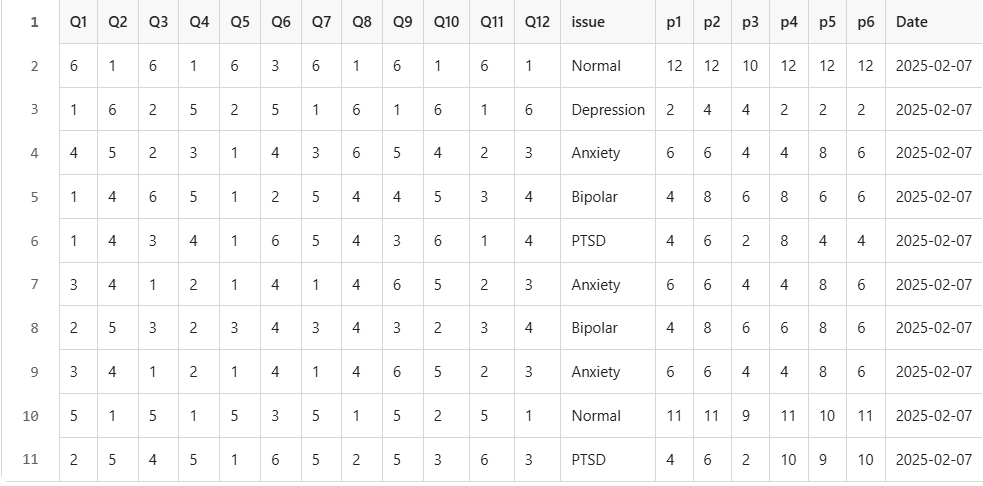
\includegraphics[width=0.8\textwidth]{App Images/32 Interface.png}  
    \caption*{Sample Response Collection Sheet}
    \label{01i}  % Label for referencing the figure
\end{figure}


\pagebreak

\begin{table}[H]
    \centering
    \caption*{Step-by-Step Algorithm for Association Matrix Analysis}
    \label{tab:algorithm}
    \begin{tabularx}{\textwidth}{|c|p{6cm}|>{\raggedright\arraybackslash}X|}
    \hline
    \textbf{Step} & \textbf{Operation} & \textbf{Mathematical Formula / Description} \\ \hline
    1 & \textbf{Load Dataset} & Read the CSV file (e.g., \texttt{am.csv}) to obtain the association matrix data. \\ \hline
    2 & \textbf{Define Row Names and Issue Columns} & Set row names: 
    \begin{tabular}[t]{@{}l@{}}self acceptance, positive relations with \\ others, autonomy, environmental mastery,\\ purpose in life, personal growth\end{tabular} \\ \hline
    3 & \textbf{Extract Association Matrix} & Let \( \displaystyle A \in \mathbb{R}^{6 \times 5}, \quad A_{ij} \text{ is the value for the } i\text{-th parameter} \) and j-th issue with issue columns ordered as: anxiety, bipolar, depression, normal, ptsd. \\ \hline
    4 & \textbf{Define Probabilities Vector} & Define the probability vector where \(I_j\) refers to the mental issue probabilities. \newline
    \( \displaystyle \vec{p} = \begin{bmatrix} I1 \\ I2 \\ I3 \\ I4 \\ I5 \end{bmatrix}, \)
    which satisfies \( \displaystyle \sum_{j=1}^{5} I_j = 1 \).\newline \\ \hline
    5 & \textbf{Weighted Sum Analysis} & Compute the weighted sum for each row: 
    \( \displaystyle w_i = \sum_{j=1}^{5} A_{ij}\, p_j, \quad i=1,\dots,6. \)
    Identify the row index with maximum \(w_i\), i.e., \( \displaystyle i^* = \arg\max_{i}\, w_i. \) \\ \hline
    6 & \textbf{Cosine Similarity Analysis} & For each row vector \( \vec{a}_i \) of \(A\), compute:
    \( \displaystyle s_i = \frac{\vec{a}_i \cdot \vec{p}}{\|\vec{a}_i\|\,\|\vec{p}\|}, \quad i=1,\dots,6. \)
    Determine \( \displaystyle i^* = \arg\max_{i}\, s_i. \) \\ \hline
    7 & \textbf{Euclidean Distance Analysis} & For each row, compute the Euclidean distance:
    \( \displaystyle d_i = \sqrt{\sum_{j=1}^{5} \left(A_{ij} - p_j\right)^2}, \quad i=1,\dots,6. \)
    Find the row index with the smallest distance:
    \( \displaystyle i^* = \arg\min_{i}\, d_i. \) \newline \\ \hline
    8 & \textbf{Consensus Decision} & Compare the row names identified by the three analyses. If all three methods return the same row name, that is the consensus; otherwise, list the unique names obtained. \\ \hline
\end{tabularx}
\end{table}

\begin{table}[H]
    \centering
    \caption*{Step-by-Step Algorithm for Association Matrix Analysis}
    \label{tab:algorithm}
    \begin{tabularx}{\textwidth}{|c|p{6cm}|>{\raggedright\arraybackslash}X|}
    \hline
    \textbf{Step} & \textbf{Operation} & \textbf{Mathematical Formula / Description} \\ \hline
    9 & \textbf{Display Results} & Use Streamlit to display:
    \begin{itemize}[noitemsep, topsep=0pt]
        \item The original Association Matrix.
        \item The computed weighted sums, cosine similarity scores, and Euclidean distances.
        \item The row(s) corresponding to the maximum weighted sum, highest cosine similarity, and smallest Euclidean distance.
        \item The consensus result.
    \end{itemize} \\ \hline
    \end{tabularx}
\end{table}

\begin{figure}[h!]  
    \centering
    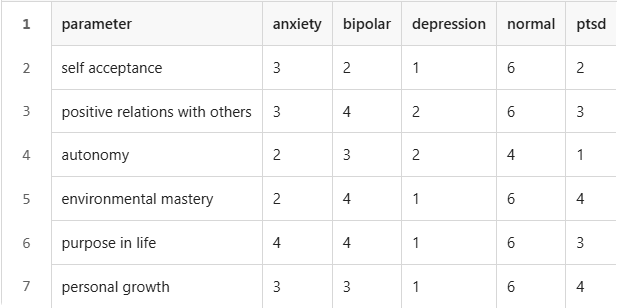
\includegraphics[width=0.65\textwidth]{App Images/33 Interface.png}  
    \caption*{Sample Association Matrix}
    \label{01i}  % Label for referencing the figure
\end{figure}


% --------- screenshots

\noindent
Below are some screenshots from the web application.

\begin{figure}[h!]  
    \centering
    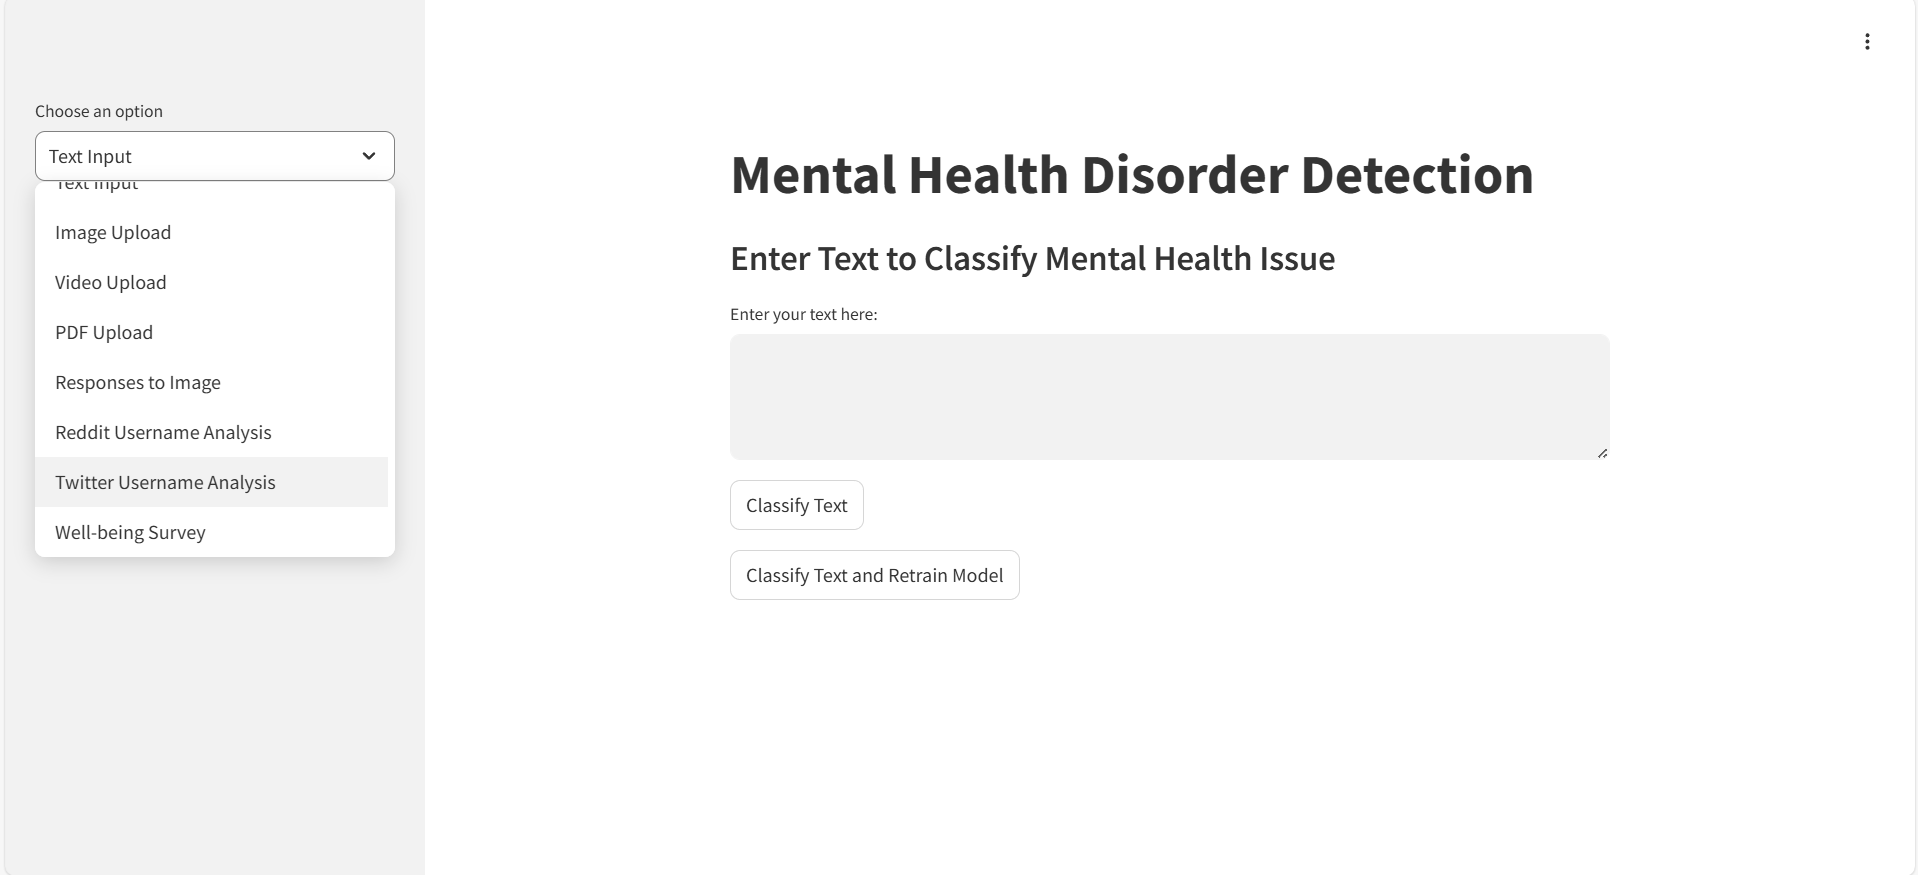
\includegraphics[width=0.9\textwidth]{App Images/01 Interface.png}  
    \caption*{Web Application Interface}
    \label{01i}  % Label for referencing the figure
\end{figure}

\pagebreak

\begin{figure}[h!]
    \centering
    % First subfigure: Text Input Option
    \begin{subfigure}[b]{0.495\textwidth}
        \centering
        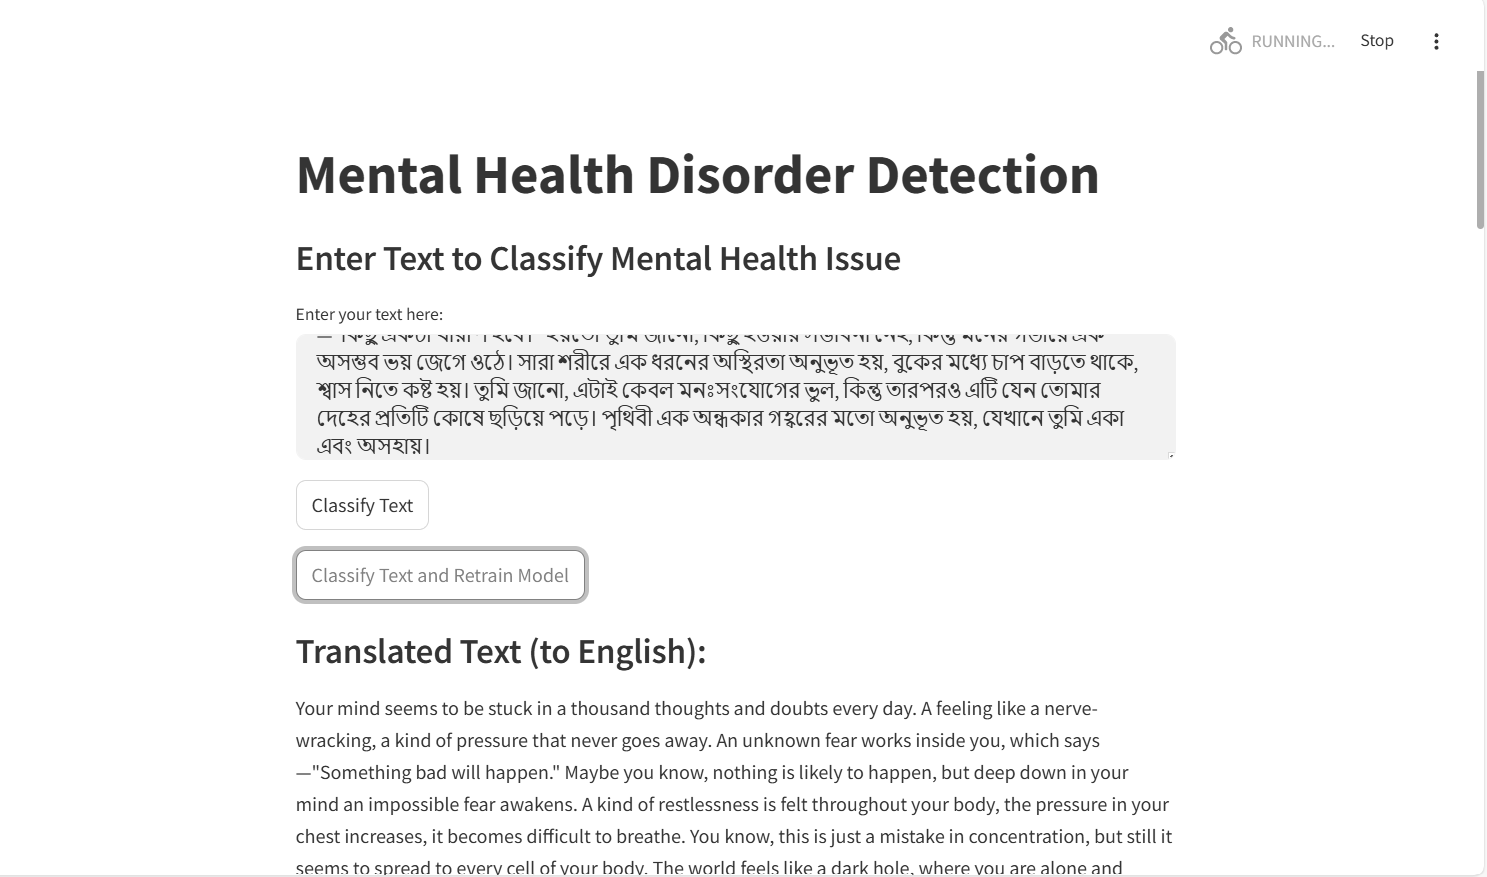
\includegraphics[width=\textwidth]{App Images/02 Interface.png}
        \caption*{Text Input Option}
        \label{fig:02i}
    \end{subfigure}
    \hfill
    % Second subfigure: Upload Image
    \begin{subfigure}[b]{0.495\textwidth}
        \centering
        
\includegraphics[width=\textwidth]{App Images/04 Interface.png}
        \caption*{Upload Image Option}
        \label{fig:04i}
    \end{subfigure}
    \label{fig:app_interfaces}
\end{figure}

\vspace{-2em}

\begin{figure}[h!]
    \centering
    % First subfigure: Upload Video
    \begin{subfigure}[b]{0.495\textwidth}
        \centering
        
\includegraphics[width=\textwidth]{App Images/12 Interface.png}
        \caption*{Upload Video Option}
        \label{fig:06i4}
    \end{subfigure}
    \hfill
    % Second subfigure: PDF Upload Option
    \begin{subfigure}[b]{0.495\textwidth}
        \centering
        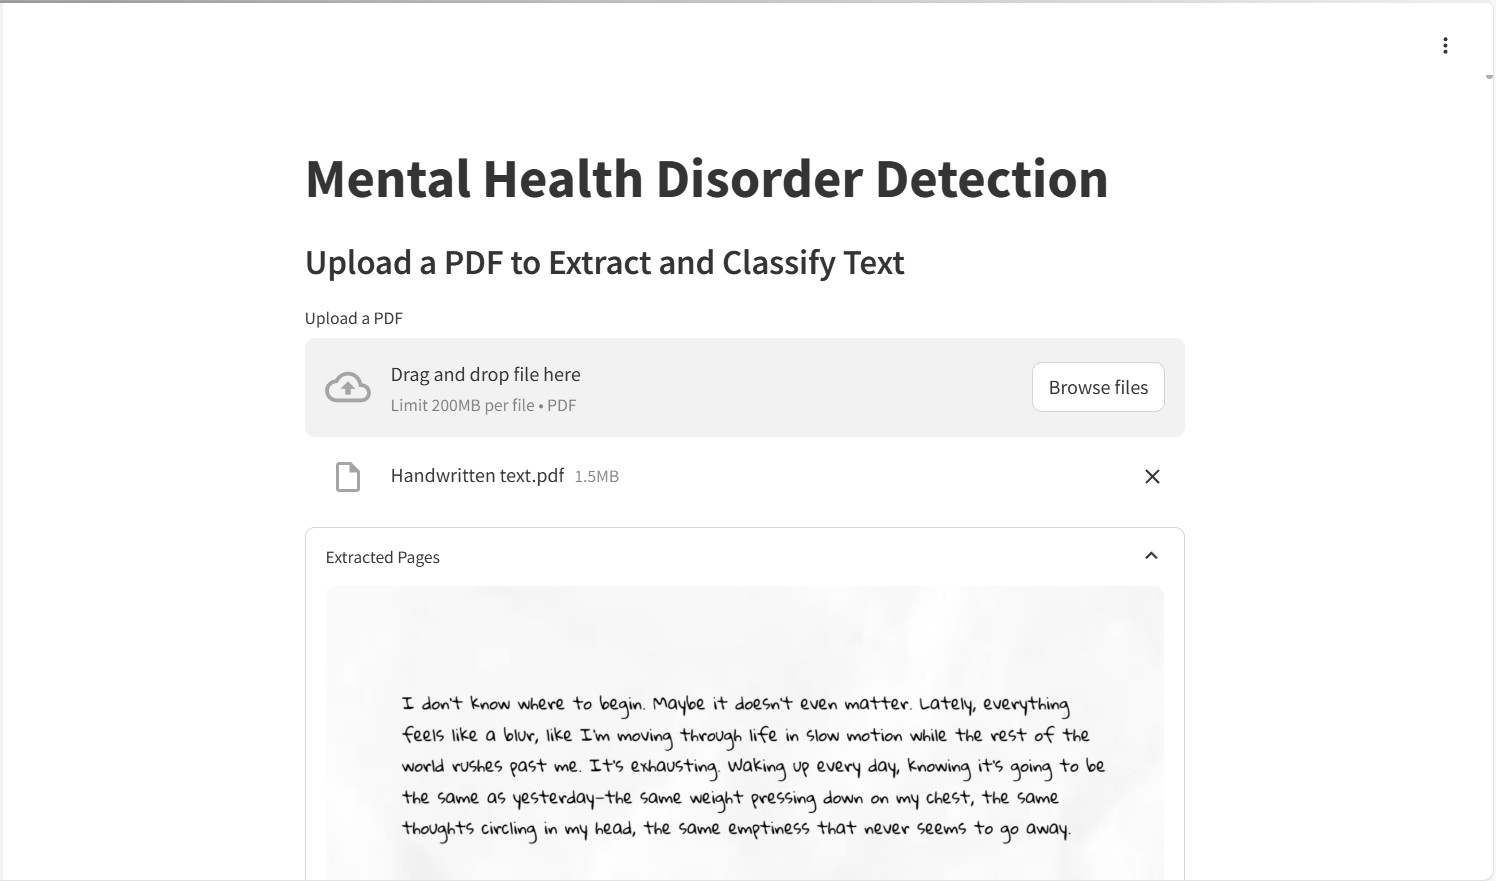
\includegraphics[width=\textwidth]{App Images/20 Interface.png}
        \caption*{PDF Upload Option}
        \label{fig:10i23445}
    \end{subfigure}
    \label{fig:app_interfaces_upload}
\end{figure}

\vspace{-2em}

\begin{figure}[h!]
    \centering
    % First subfigure: User response to Image Option
    \begin{subfigure}[b]{0.495\textwidth}
        \centering
        
\includegraphics[width=\textwidth]{App Images/26 Interface.png}
        \caption*{User response to Image Option}
        \label{fig:26Interface}
    \end{subfigure}
    \hfill
    % Second subfigure: Questions related to image
    \begin{subfigure}[b]{0.495\textwidth}
        \centering
        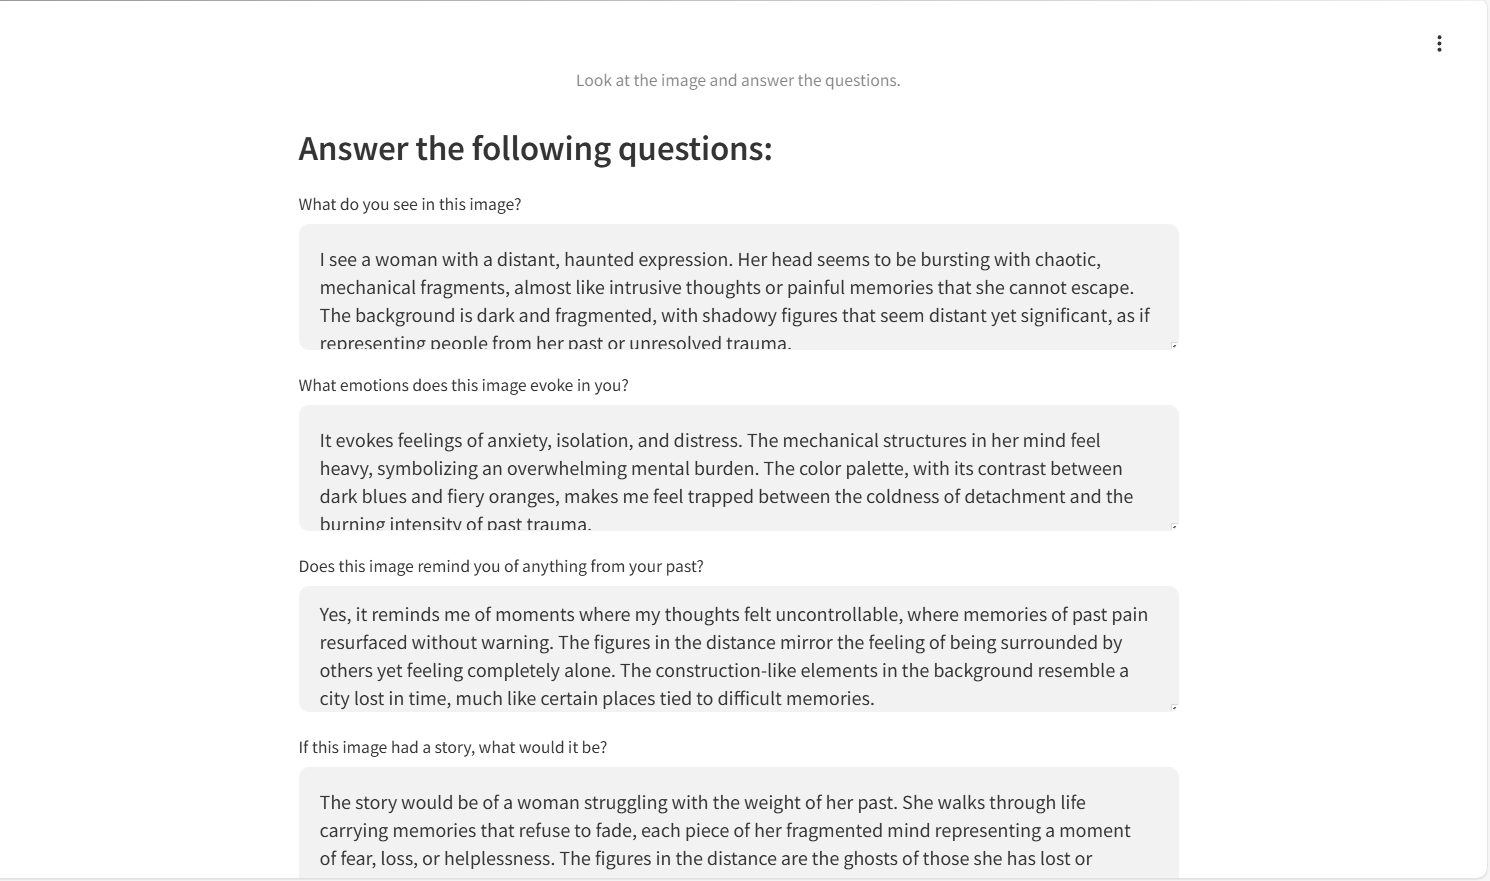
\includegraphics[width=\textwidth]{App Images/27 Interface.png}
        \caption*{Questions related to image}
        \label{fig:27Interface}
    \end{subfigure}
    \label{fig:imageResponseAndQuestions}
\end{figure}

\vspace{-2em}

\begin{figure}[H]
    \centering
    % First subfigure: Reddit User Analysis
    \begin{subfigure}[b]{0.495\textwidth}
        \centering
        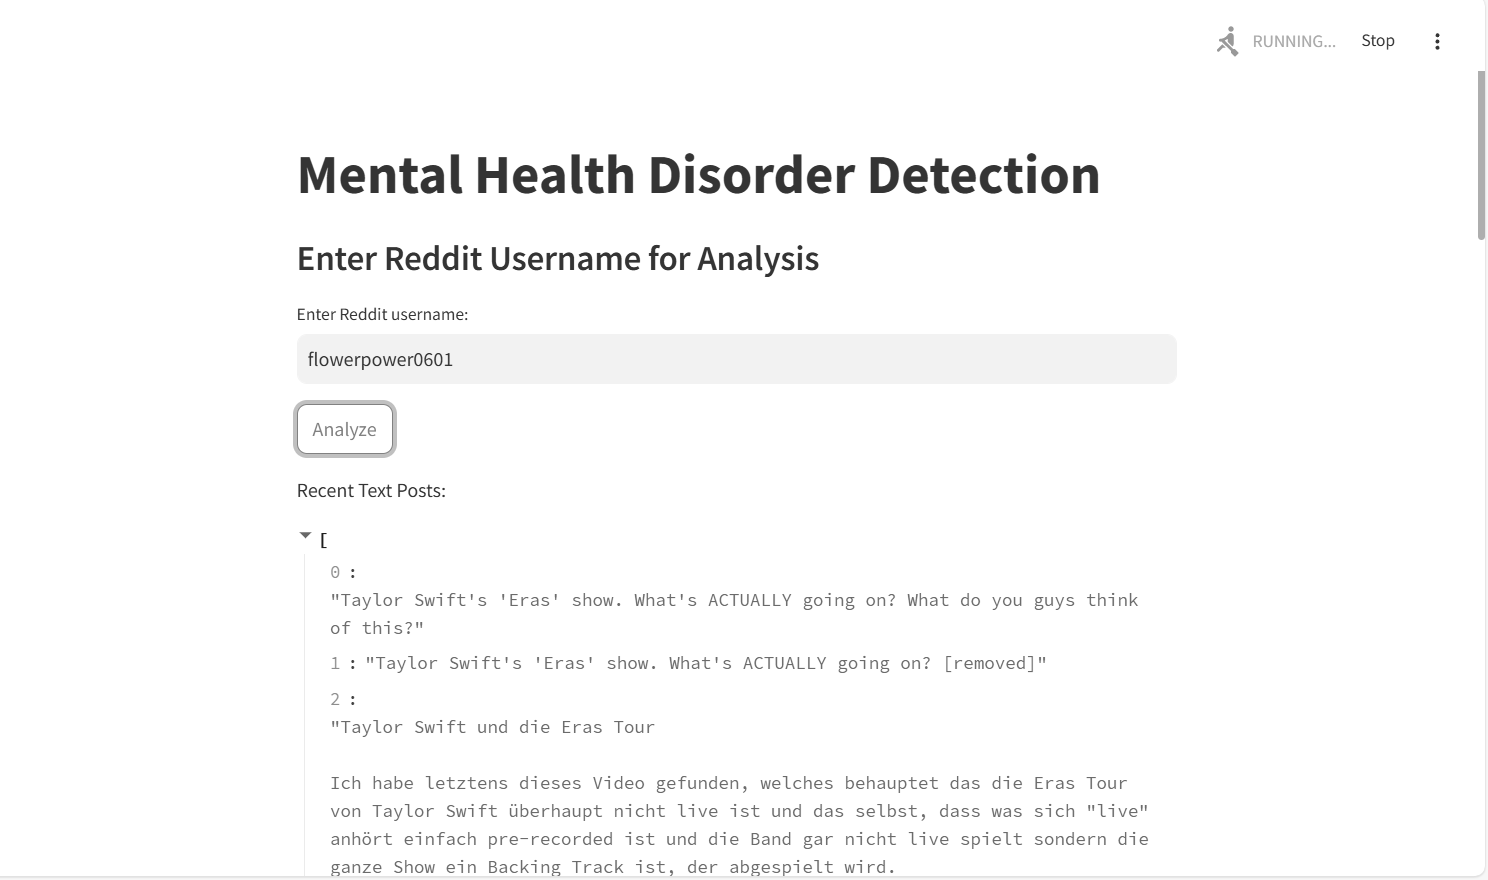
\includegraphics[width=\textwidth]{App Images/06 Interface.png}
        \caption*{Reddit User Analysis Option}
        \label{fig:07i}
    \end{subfigure}
    \hfill
    % Second subfigure: Twitter User Analysis
    \begin{subfigure}[b]{0.495\textwidth}
        \centering
        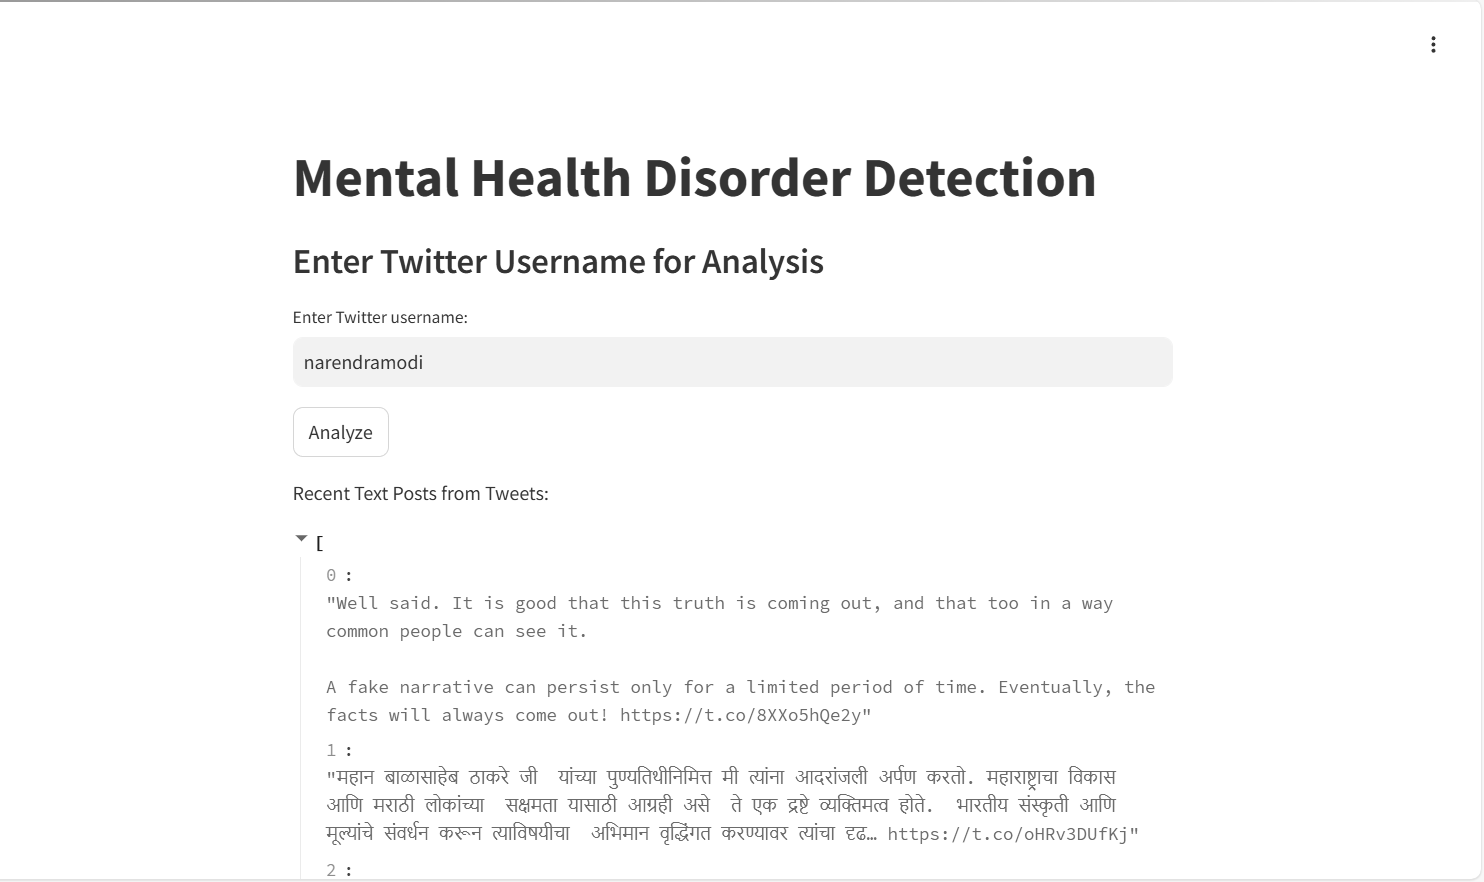
\includegraphics[width=\textwidth]{App Images/08 Interface.png}
        \caption*{Twitter User Analysis Option}
        \label{fig:09i}
    \end{subfigure}
    \label{fig:reddit_twitter_analysis}
\end{figure}

\pagebreak

\begin{figure}[h!]
    \centering
    % First subfigure: Prediction and Insights
    \begin{subfigure}[b]{0.495\textwidth}
        \centering
        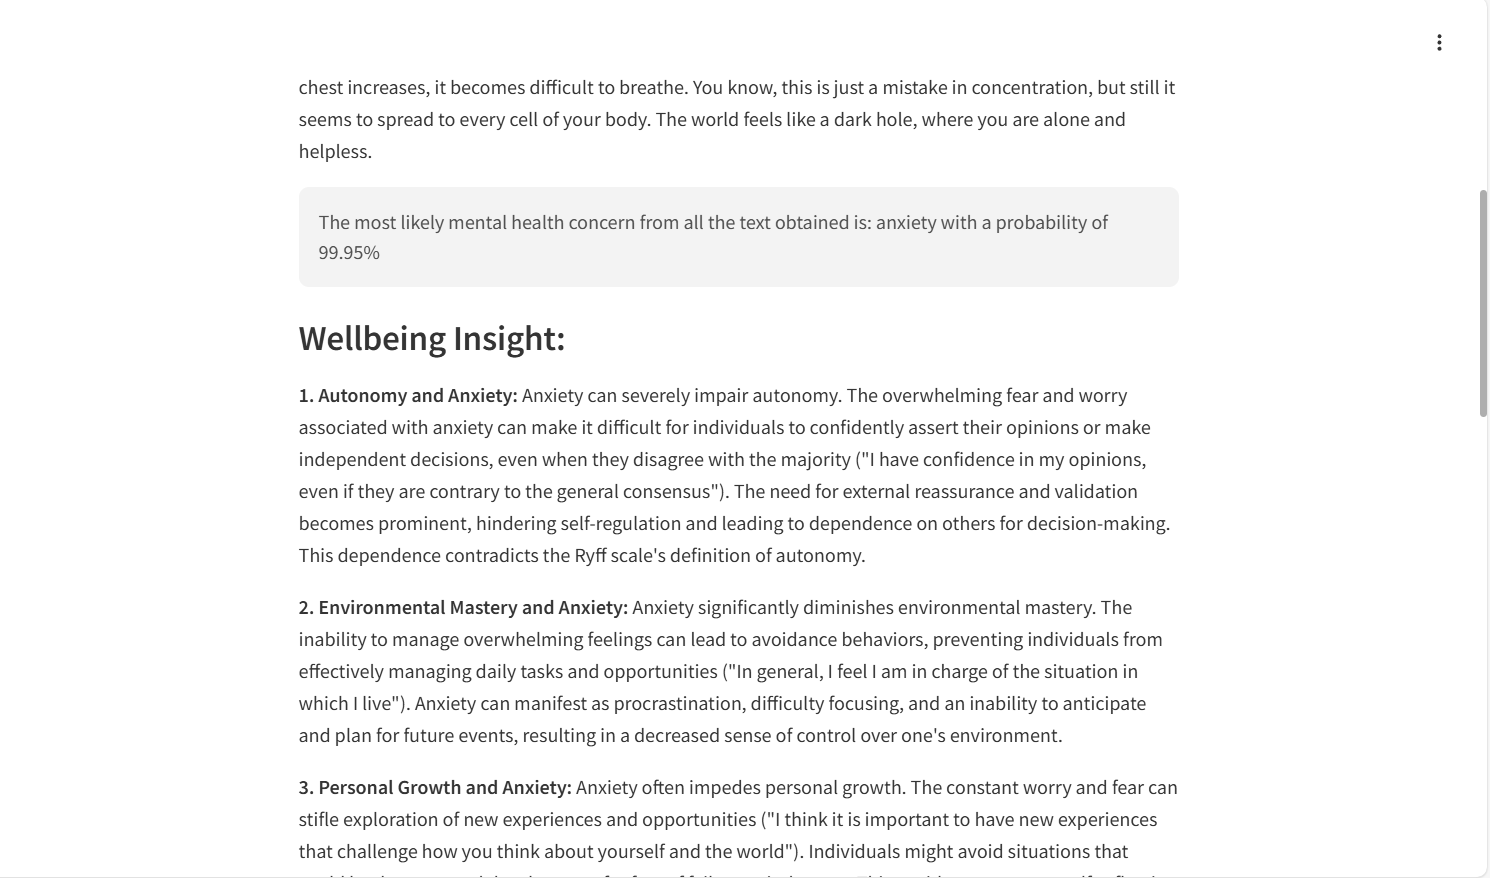
\includegraphics[width=\textwidth]{App Images/03 Interface.png}
        \caption*{Prediction and Insights}
        \label{fig:03i}
    \end{subfigure}
    \hfill
    % Second subfigure: Social Media User Analysis
    \begin{subfigure}[b]{0.495\textwidth}
        \centering
        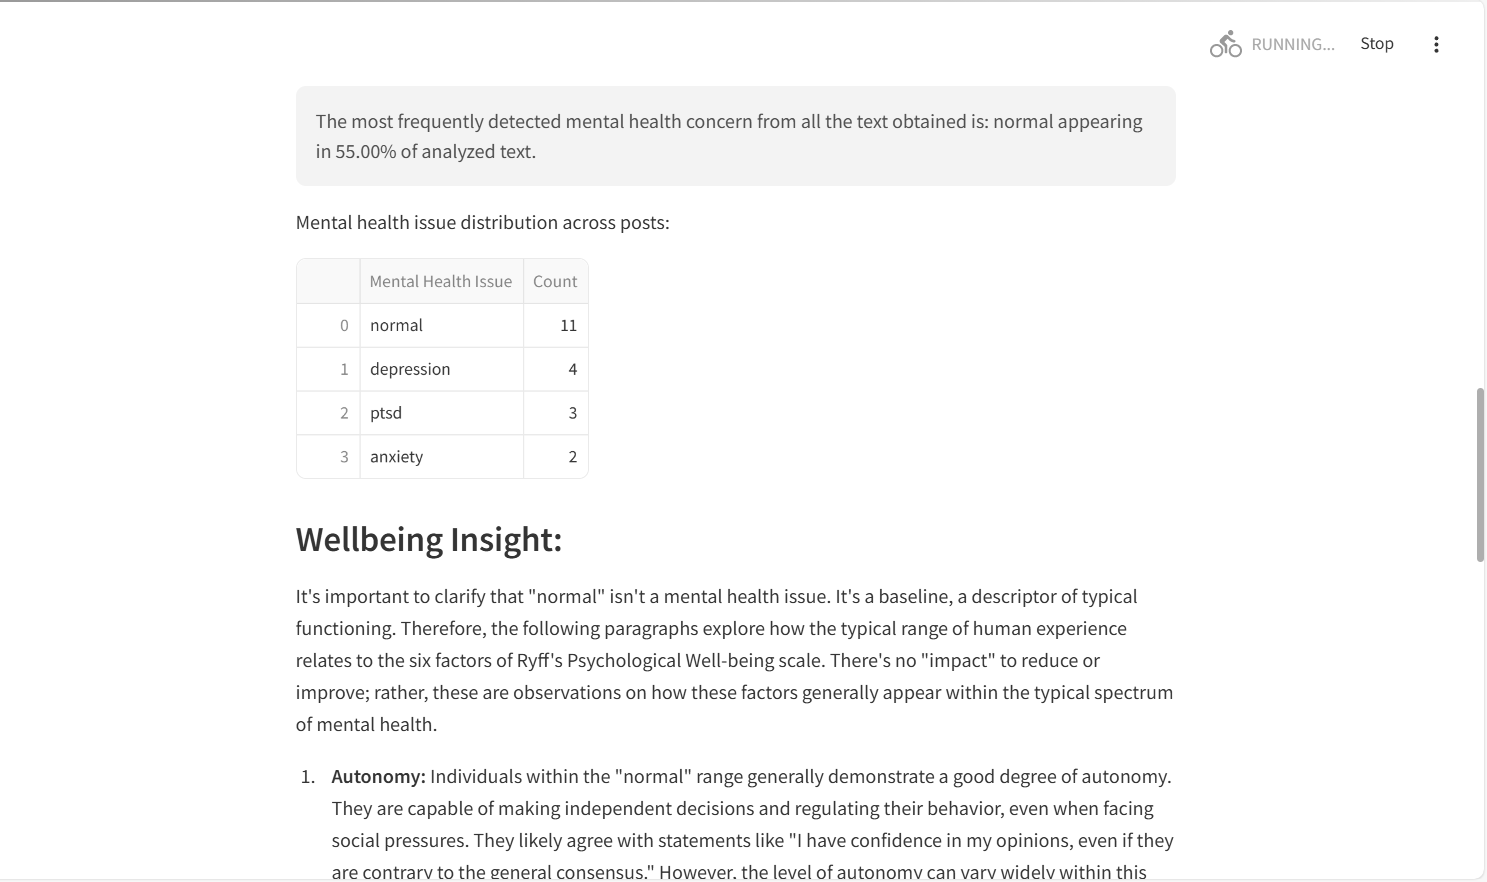
\includegraphics[width=\textwidth]{App Images/07 Interface.png}
        \caption*{Social Media User Analysis}
        \label{fig:08i}
    \end{subfigure}
    \label{fig:combined_analysis}
\end{figure}

\vspace{-2em}

\begin{figure}[h!]
    \centering
    % First subfigure: Model Retraining Result
    \begin{subfigure}[b]{0.495\textwidth}
        \centering
        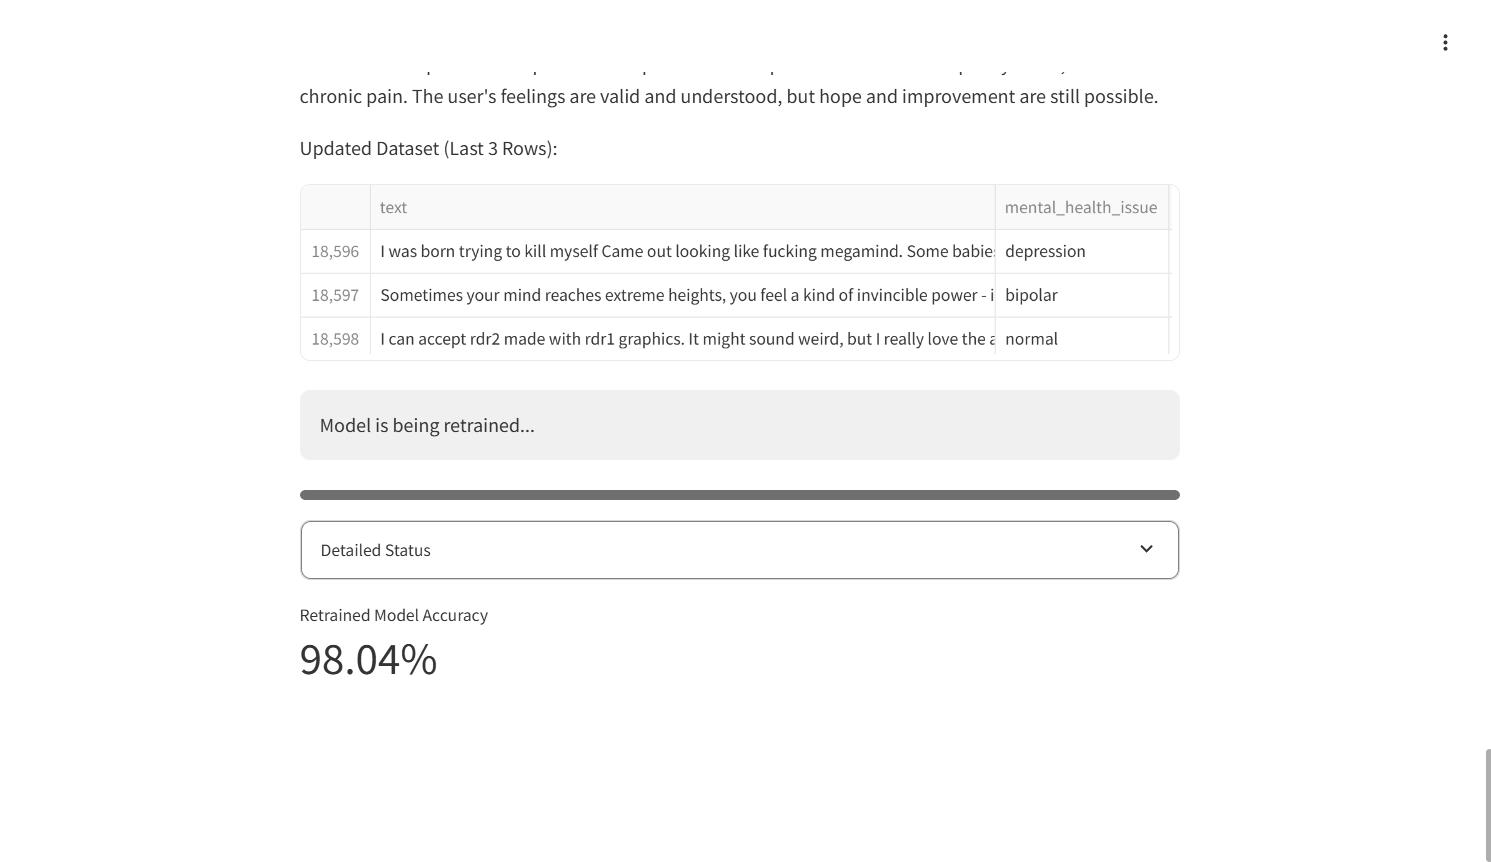
\includegraphics[width=\textwidth]{App Images/17 Interface.png}
        \caption*{Model Retraining Result}
        \label{fig:10i}
    \end{subfigure}
    \hfill
    % Second subfigure: Emotion analysis
    \begin{subfigure}[b]{0.495\textwidth}
        \centering
        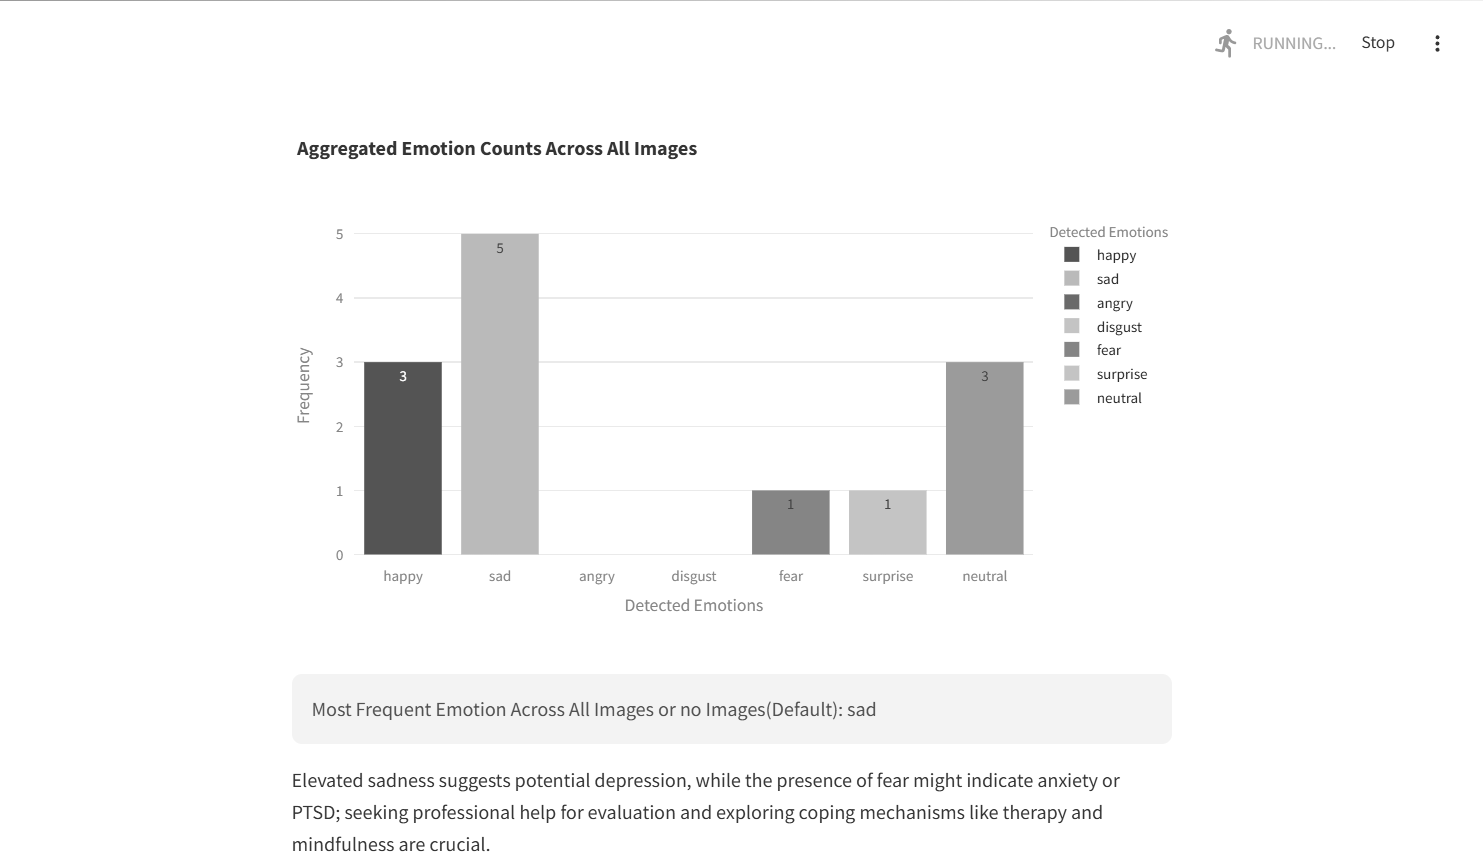
\includegraphics[width=\textwidth]{App Images/12-1 Interface.png}
        \caption*{Emotion analysis}
        \label{fig:10i23}
    \end{subfigure}
    \label{fig:comparison}
\end{figure}

\vspace{-2em}

\begin{figure}[h!]
    \centering
    % First subfigure: Generate Image Caption
    \begin{subfigure}[b]{0.495\textwidth}
        \centering
        
\includegraphics[width=\textwidth]{App Images/18 Interface.png}
        \caption*{Generate Image Caption}
        \label{fig:10i234}
    \end{subfigure}
    \hfill
    % Second subfigure: Knowledge Graph after prediction
    \begin{subfigure}[b]{0.495\textwidth}
        \centering
        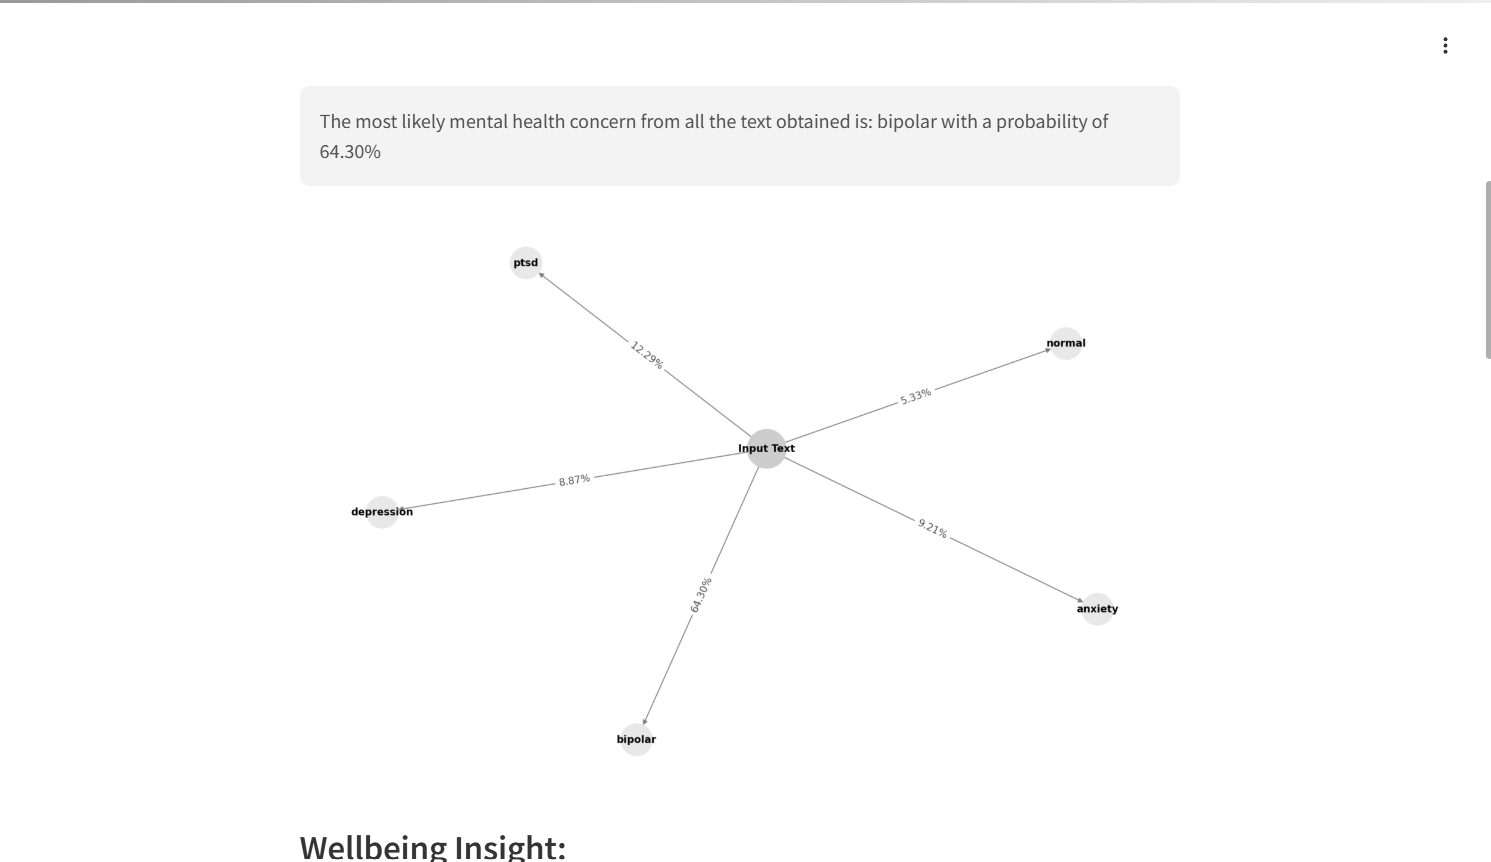
\includegraphics[width=\textwidth]{App Images/19 Interface.png}
        \caption*{Knowledge Graph after prediction}
        \label{fig:10i23445}
    \end{subfigure}
    \label{fig:generated_caption_vs_kg}
\end{figure}

\vspace{-2em}

\begin{figure}[H]
    \centering
    % First subfigure: Weighted Sum Analysis
    \begin{subfigure}[b]{0.495\textwidth}
        \centering
        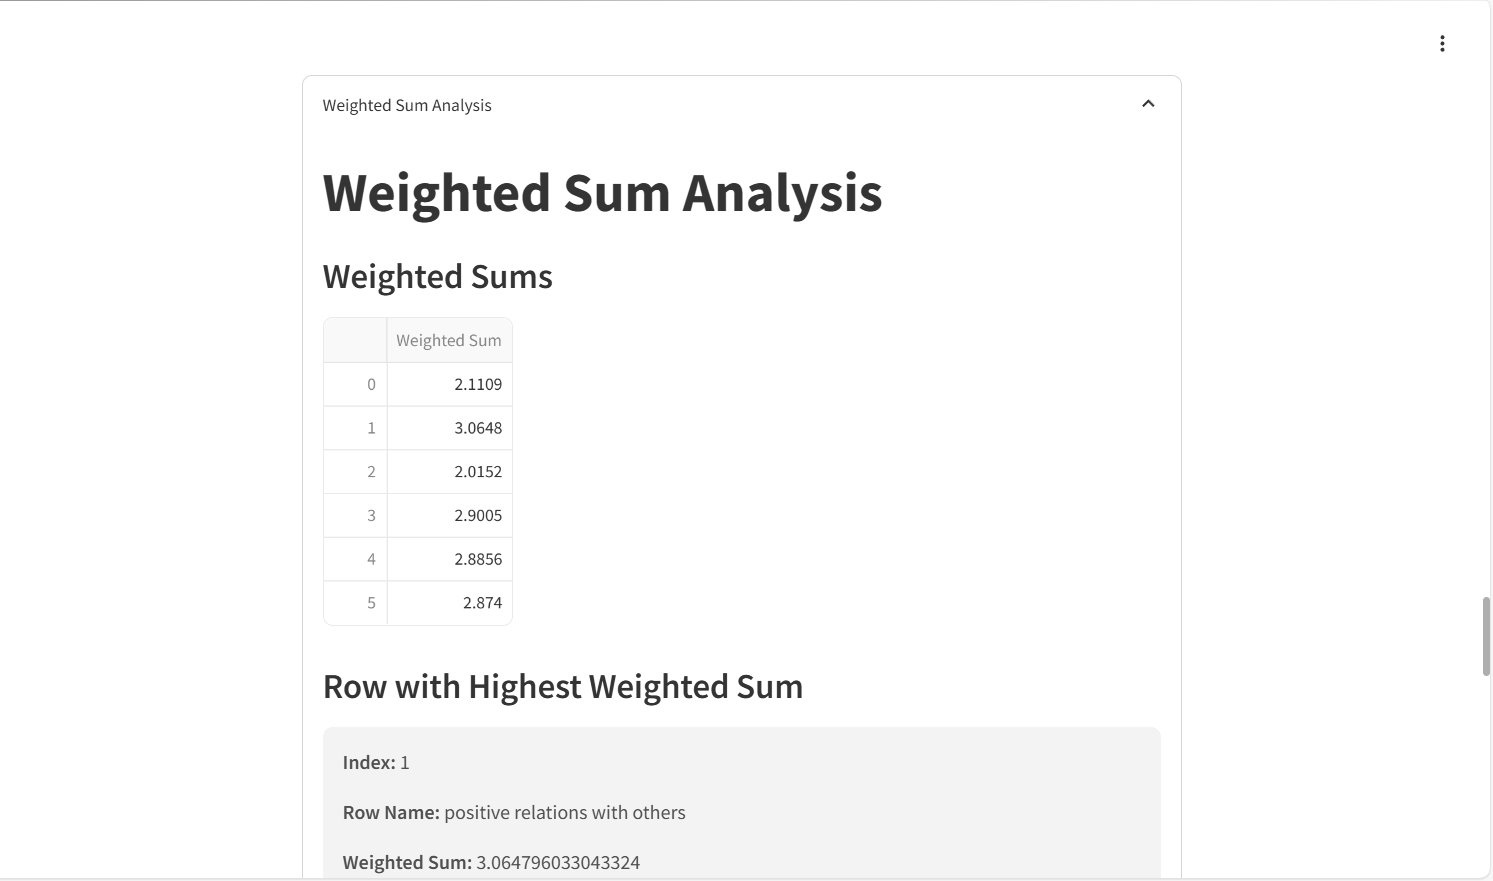
\includegraphics[width=\textwidth]{App Images/22 Interface.png}
        \caption*{Weighted Sum Analysis}
        \label{fig:weighted_sum}
    \end{subfigure}
    \hfill
    % Second subfigure: Cosine Similarity Analysis
    \begin{subfigure}[b]{0.495\textwidth}
        \centering
        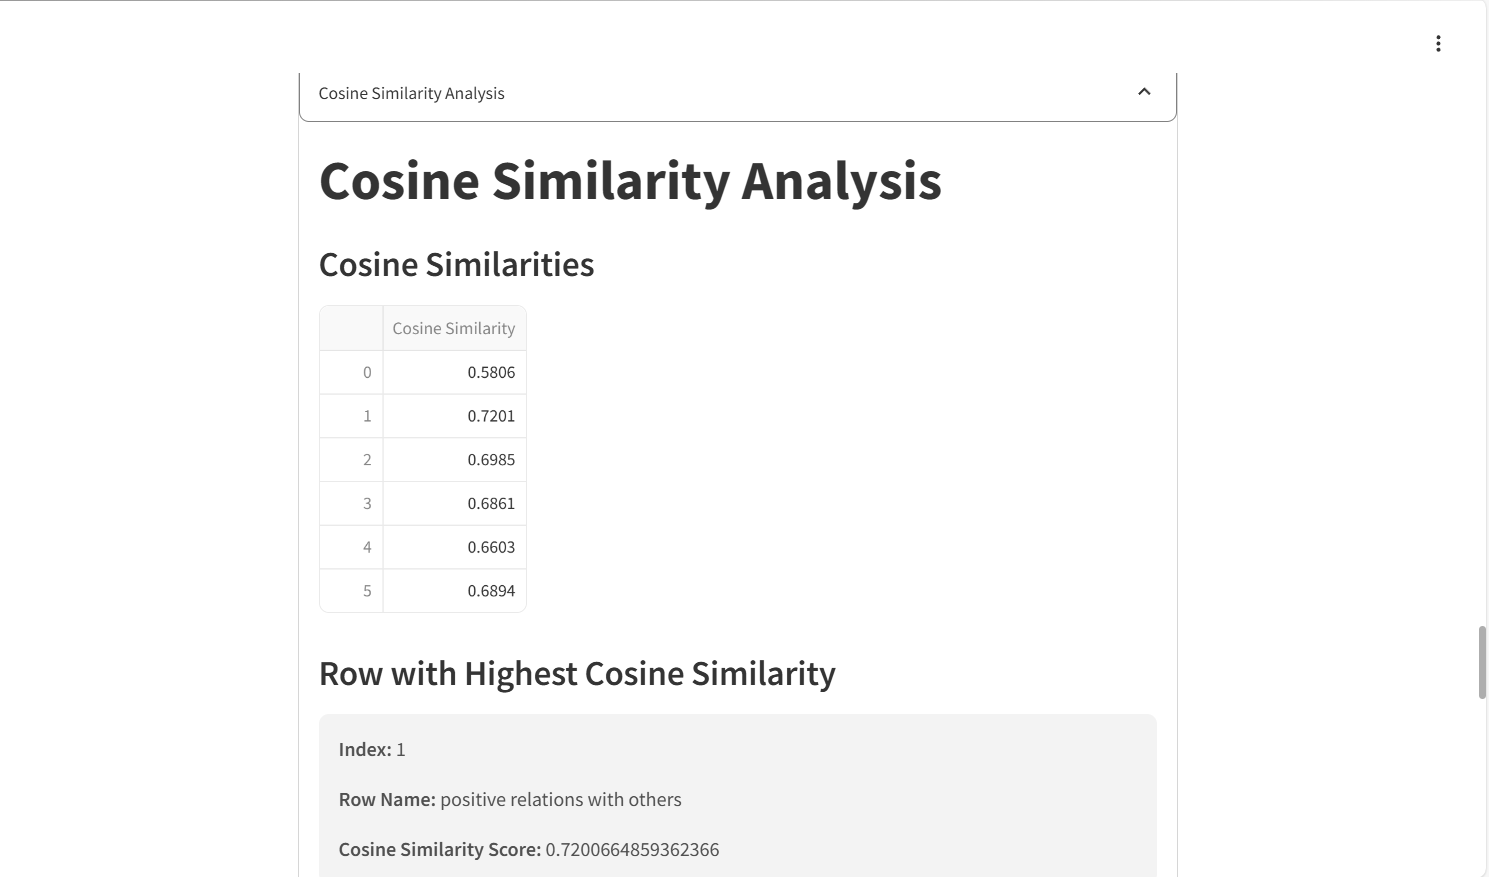
\includegraphics[width=\textwidth]{App Images/23 Interface.png}
        \caption*{Cosine Similarity Analysis}
        \label{fig:cosine_similarity}
    \end{subfigure}
    \label{fig:analysis_comparison}
\end{figure}

\pagebreak

\begin{figure}[h!]
    \centering
    % First subfigure: Euclidean Distance Analysis
    \begin{subfigure}[b]{0.495\textwidth}
        \centering
        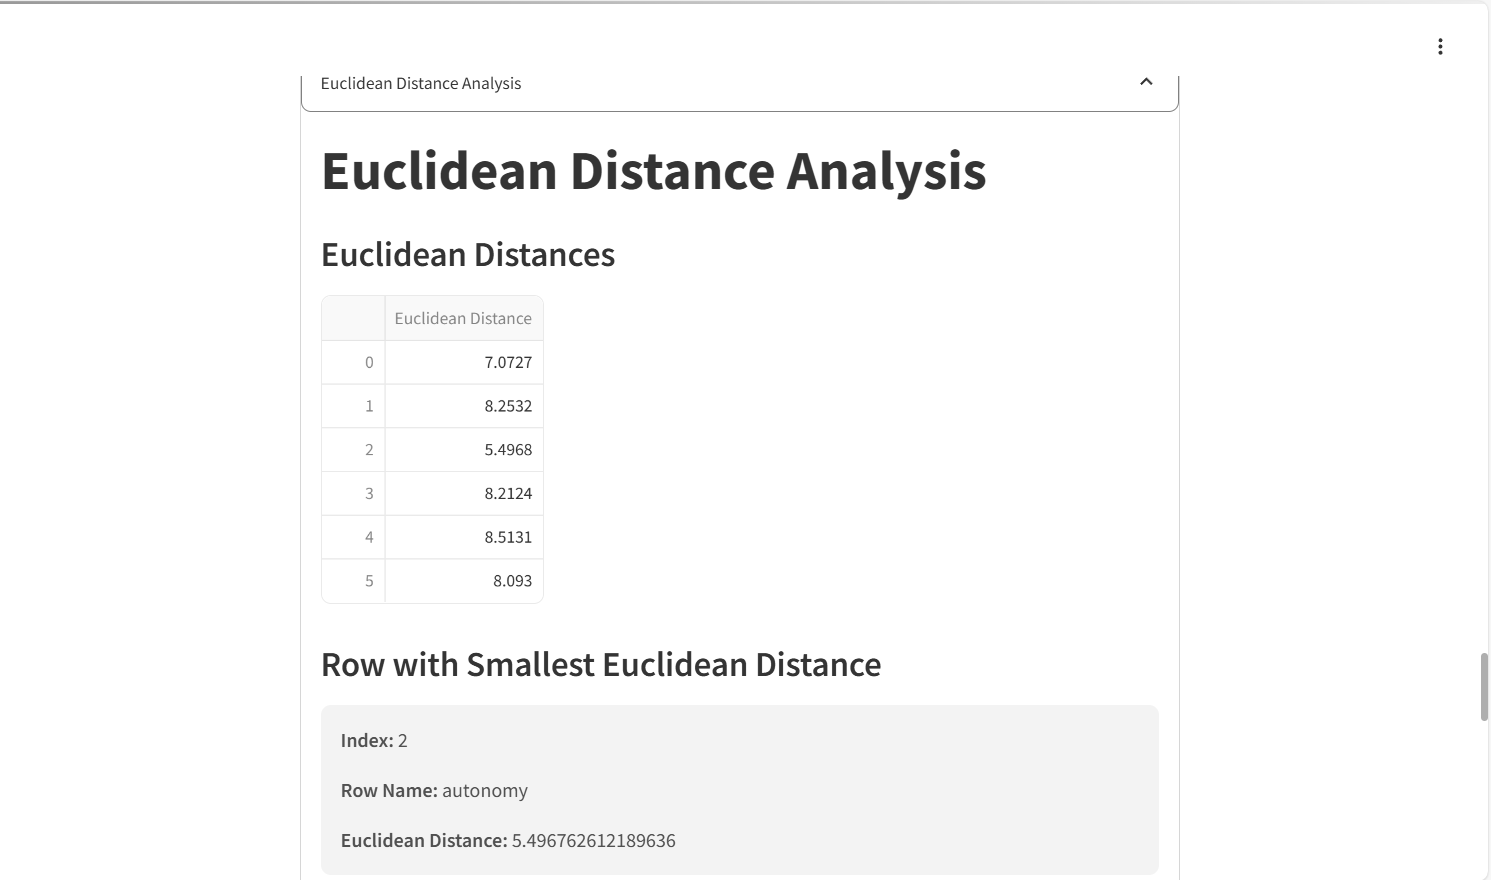
\includegraphics[width=\textwidth]{App Images/24 Interface.png}
        \caption*{Euclidean Distance Analysis}
        \label{fig:euclidean_distance}
    \end{subfigure}
    \hfill
    % Second subfigure: Specific Parameter based Insights
    \begin{subfigure}[b]{0.495\textwidth}
        \centering
        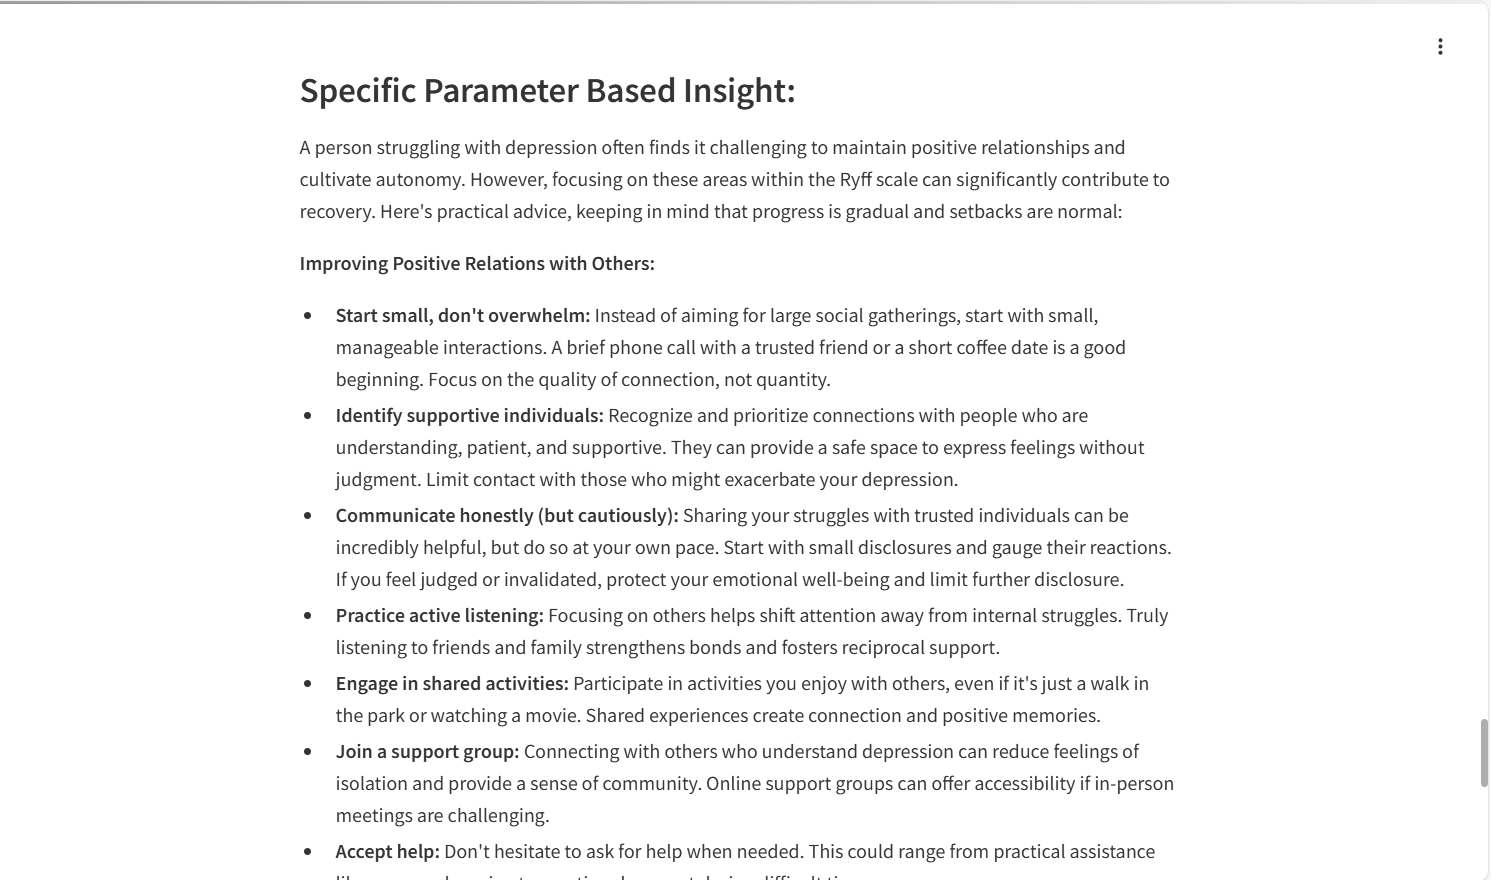
\includegraphics[width=\textwidth]{App Images/25 Interface.png}
        \caption*{Specific Parameter based Insights}
        \label{fig:specific_insights}
    \end{subfigure}
    \label{fig:analysis_comparison}
\end{figure}

\vspace{-2em}

\begin{figure}[h!]
    \centering
    % First subfigure: Well-being survey questions
    \begin{subfigure}[b]{0.495\textwidth}
        \centering
        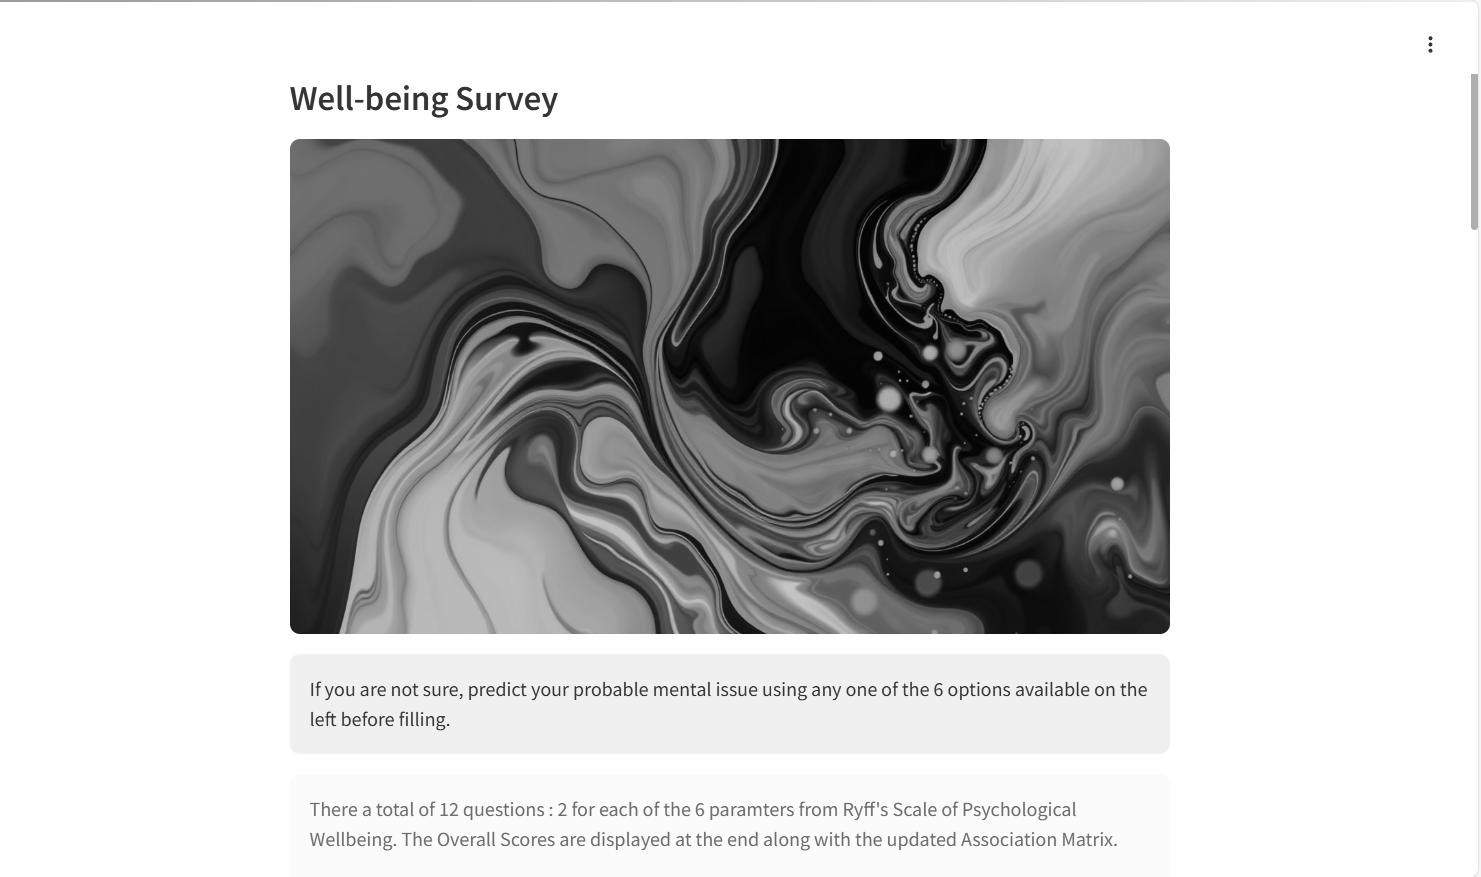
\includegraphics[width=\textwidth]{App Images/28 Interface.png}
        \caption*{Well-being survey option}
        \label{fig:wellbeing_questions}
    \end{subfigure}
    \hfill
    % Second subfigure: Well-being survey result
    \begin{subfigure}[b]{0.495\textwidth}
        \centering
        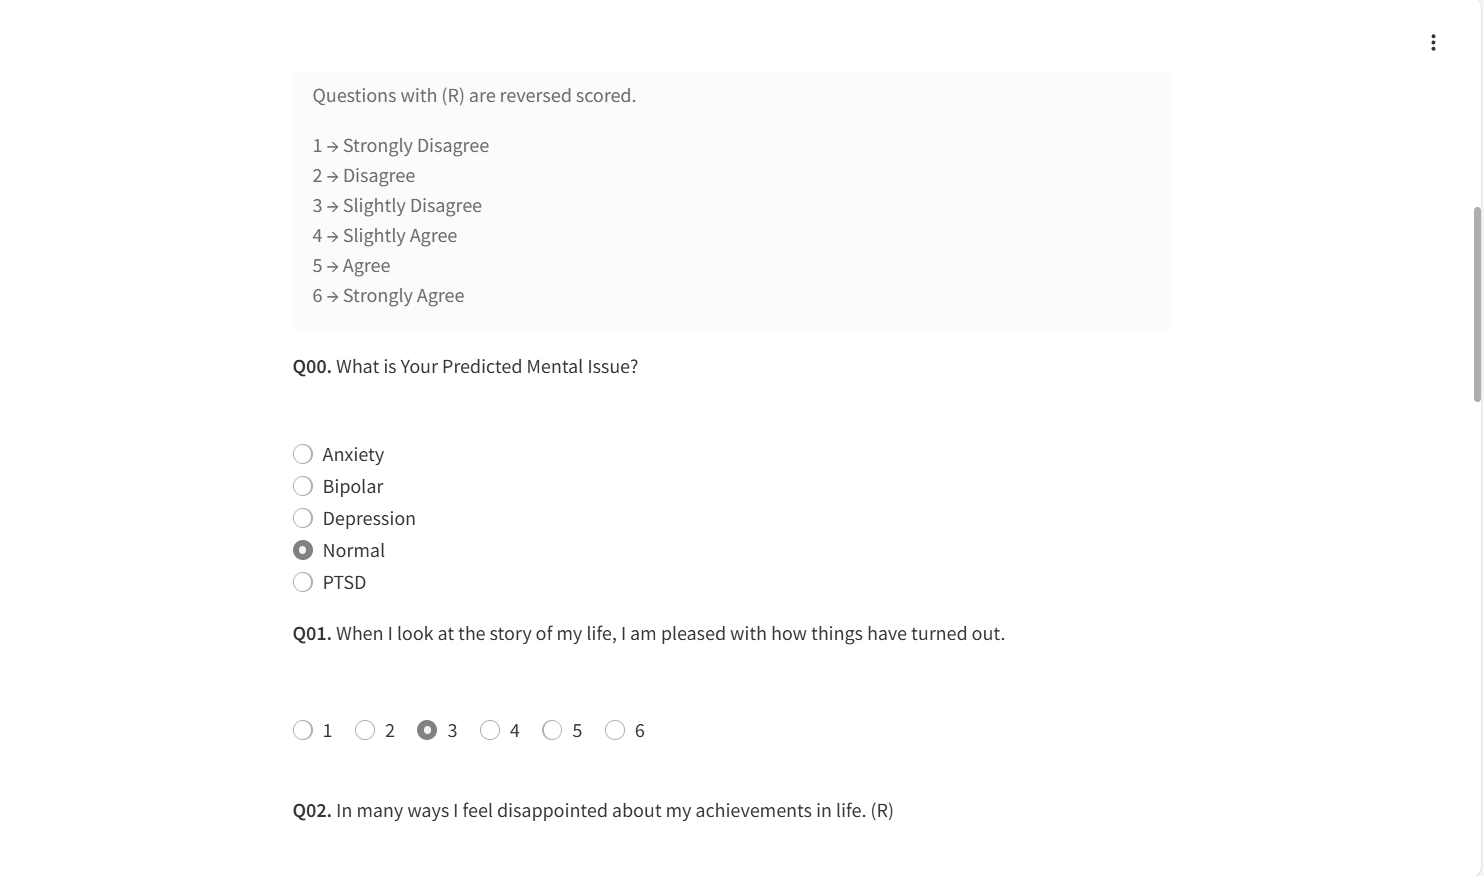
\includegraphics[width=\textwidth]{App Images/29 Interface.png}
        \caption*{Well-being survey questions}
        \label{fig:wellbeing_result}
    \end{subfigure}
    \label{fig:wellbeing_comparison}
\end{figure}

\vspace{-2em}

\begin{figure}[h!]
    \centering
    % First subfigure: Well-being survey questions
    \begin{subfigure}[b]{0.495\textwidth}
        \centering
        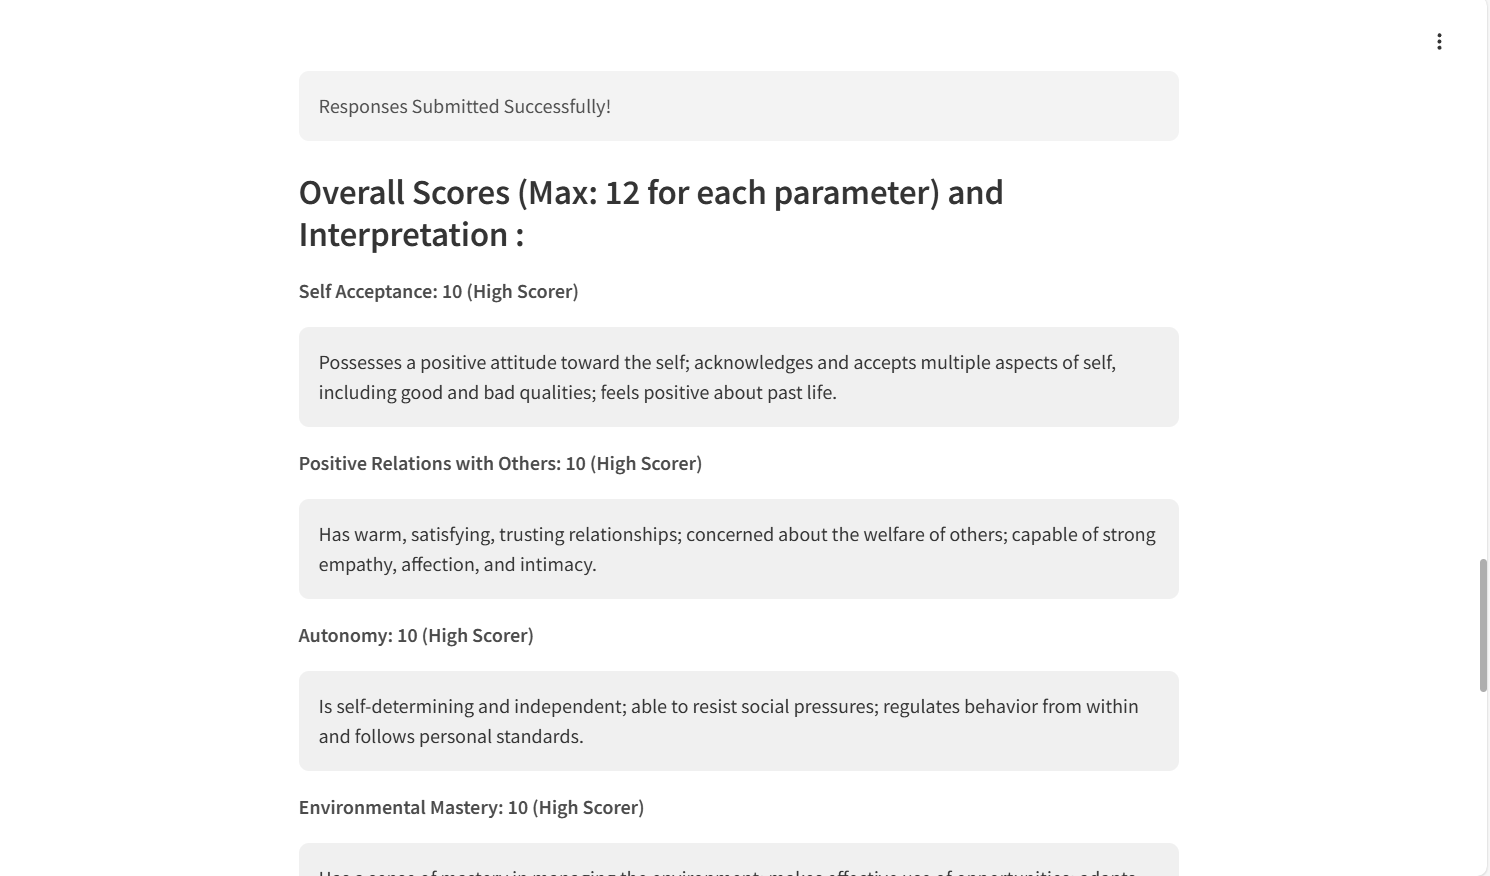
\includegraphics[width=\textwidth]{App Images/30 Interface.png}
        \caption*{Well-being survey result}
        \label{fig:wellbeing_questions}
    \end{subfigure}
    \hfill
    % Second subfigure: Well-being survey result
    \begin{subfigure}[b]{0.495\textwidth}
        \centering
        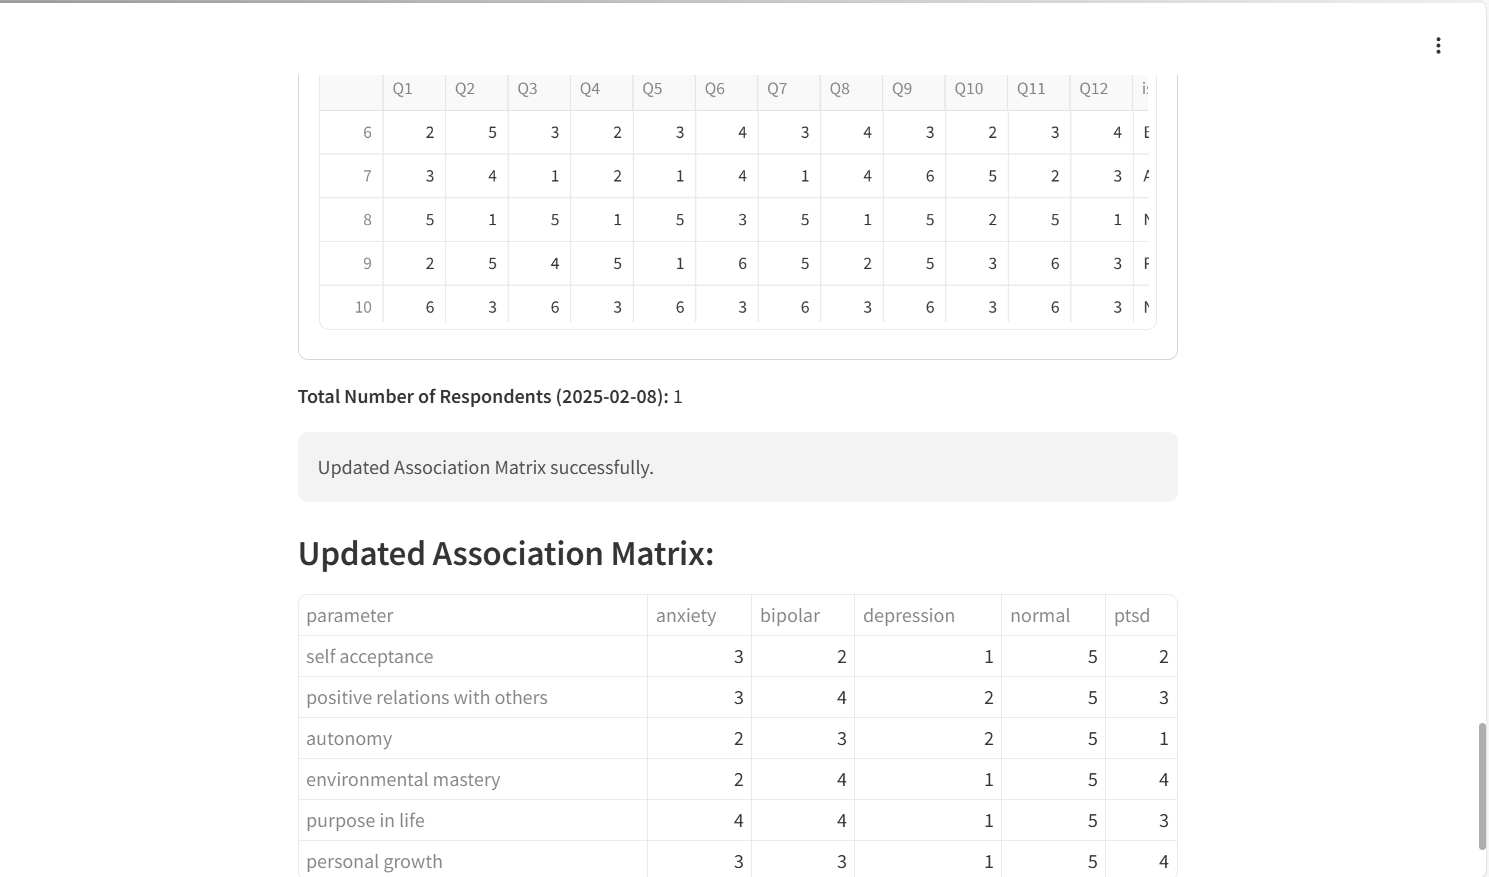
\includegraphics[width=\textwidth]{App Images/31 Interface.png}
        \caption*{Updated Association Matrix after responses}
        \label{fig:wellbeing_result}
    \end{subfigure}
    \label{fig:wellbeing_comparison}
\end{figure}

% ----------------------- Prototype ends -------------------


\begin{comment}

    \section*{APPENDIX B - Paper publications (optional) \label{sec:pubs}}
\addcontentsline{toc}{section}{APPENDIX B - Paper publications (optional)}
If any of your related paper(s) were published in a standard journal / presented in a recognized conference, mention the same including communication on your paper(s) acceptance / publishing note. You should also show appropriate documentation at the time of project viva.


\end{comment}
